% =============================================================================
%   Chapter 5: Quasi-Geostrophic Analysis
%   Based on Ch05 lecture notes (133 slides)
%   Reference: Holton and Hakim, Ch. 6; Vallis, Ch. 5
% =============================================================================

\section{Observed Structure of Extratropical Circulation}\label{sec:qg-obs}

Quasi-geostrophic (QG) theory의 수학적 체계를 전개하기 전에, 이를 동기 부여하는 관측적 특징을 간략히 살펴본다.
온대 대기는 시공간적으로 강한 \textgr{asymmetries}를 보인다: synoptic disturbances는 균일하게 분포하지 않고,
시간 평균 zonal wind가 가장 강한 영역과 일치하는 \textbf{storm tracks}에 집중된다.

\hisu{경압 불안정 = 중위도 종관 규모 시스템의 주요 불안정 메커니즘}

\begin{figure}[htbp]
  \centering
  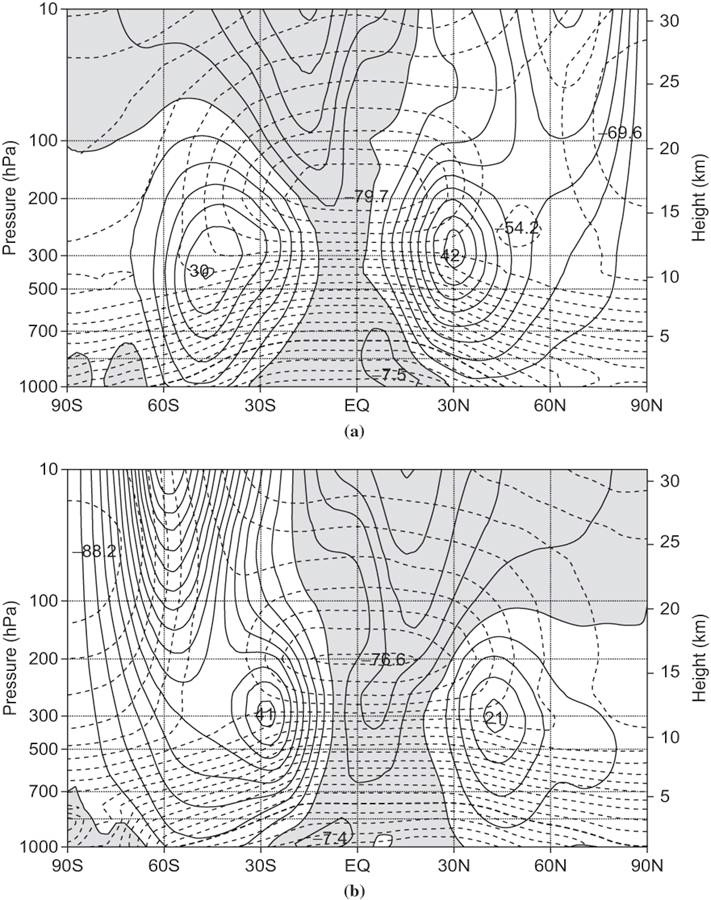
\includegraphics[width=0.85\textwidth]{images/ch05/p05_img01.jpeg}
  \caption{Observed zonally averaged cross-sections of (a)~zonal wind $\bar{u}$
    and (b)~temperature $\bar{T}$ (DJF climatology).  Solid contours denote
    westerlies / higher temperatures; dashed contours denote easterlies /
    lower temperatures.  Note the subtropical jet maxima near 200\,hPa and
    the strong meridional temperature gradient in the midlatitudes.
    \hisu{관측된 동서 평균 바람과 온도의 남북--연직 단면.
          중위도의 강한 자오 온도 경도와 아열대 제트가 경압 불안정의 배경이 된다.}}
  \label{fig:obs-zonal-uT}
\end{figure}

% --------------------------------------------------------------------------
\subsection{Storm Tracks and Jet Streams}
% --------------------------------------------------------------------------

Synoptic-scale disturbances---중위도의 이동성 cyclones와 anticyclones---는
\textgr{maximum time-mean zonal wind} 영역, 즉 서태평양 제트와 북대서양 제트 부근에서
우선적으로 발달한다.  이러한 transient eddy activity가 강화된 영역을 \textbf{storm tracks}라 한다.

\begin{remark}[Properties of Storm Tracks]
\begin{itemize}
  \item Storm tracks는 가장 강한 \textgr{baroclinicity}
        (meridional temperature gradient / vertical wind shear) 하류에 위치한다.
  \item 국지적 baroclinic energy conversion과 하류 energy propagation의 조합에 의해 유지된다.
  \item 겨울에 meridional temperature gradients가 가장 크므로 겨울에 가장 강하다.
\end{itemize}
\end{remark}

\begin{hisublock}
Storm track는 시간 평균 제트 부근에서 발생한다.
서태평양과 북대서양의 제트가 가장 강하므로, 여기에서 종관 규모 요란이
가장 활발하다.  겨울에 자오 온도 경도가 크므로 storm track도 겨울에 가장 강하다.
\end{hisublock}

\begin{figure}[htbp]
  \centering
  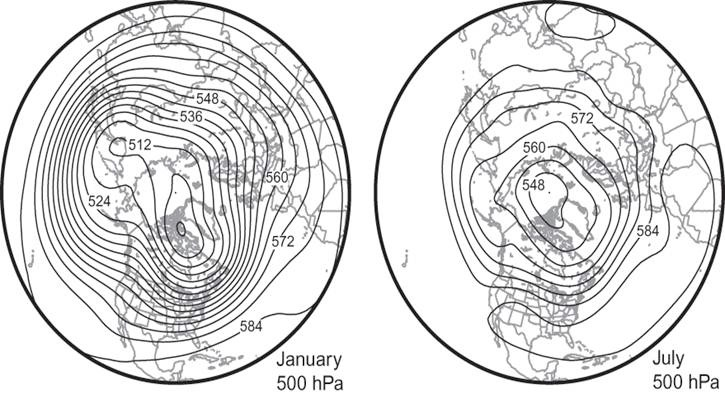
\includegraphics[width=0.85\textwidth]{images/ch05/p10_img01.jpeg}
  \caption{Time-mean 500\,hPa geopotential height for January (left) and
    July (right) over the Northern Hemisphere.  The deep troughs over
    eastern North America and eastern Asia in January mark the entrance
    regions of the major storm tracks.
    \hisu{1월과 7월의 500\,hPa 시간 평균 지위고도.
          겨울에 동아시아와 북미 동해안의 깊은 기압골이 storm track 입구를 표시한다.}}
  \label{fig:nh-500hpa-height}
\end{figure}

\begin{figure}[htbp]
  \centering
  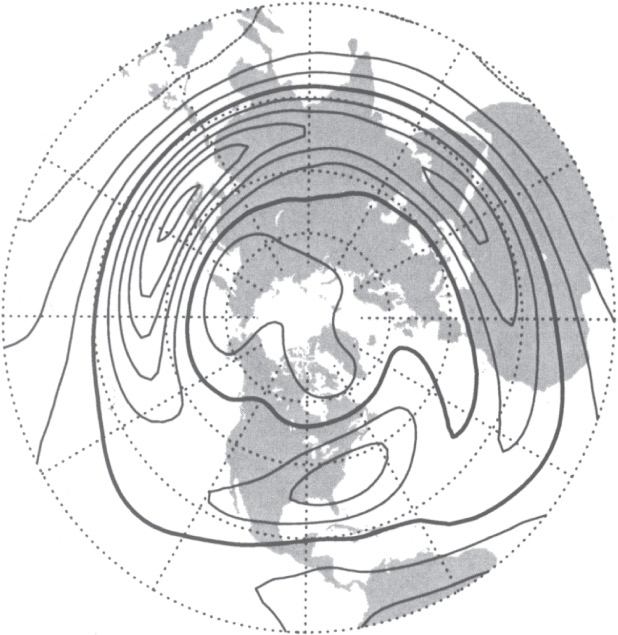
\includegraphics[width=0.4\textwidth]{images/ch05/p07_img01.jpeg}
  \caption{Northern Hemisphere mean 500\,hPa geopotential height showing
    the planetary-scale wave pattern.  Contours illustrate the quasi-stationary
    Rossby wave troughs and ridges that steer synoptic disturbances.
    \hisu{북반구 평균 500\,hPa 지위고도: 행성 규모 정상 로스비파의 기압골/기압능 패턴.}}
  \label{fig:nh-500hpa-mean}
\end{figure}

\begin{hisublock}
\textbf{참고 문헌 가이드:}
\begin{itemize}
  \item Blackmon (1977), Lau (1978, 1979) -- storm track의 관측적 정의 및 통계적 특성
  \item Hartmann (1994), \textit{Global Physical Climatology}, Ch.~6.3 (book pp.~138--149; 본 PDF에는 목차만 수록) -- 에디에 의한 에너지의 meridional transport와 storm track 유지
  \item Marshall \& Plumb (2008), \textit{Atmosphere, Ocean, and Climate Dynamics}, Ch.~8.2.2 (pp.~145--148, PDF pp.~166--169) -- extratropical circulation과 baroclinic instability의 GFD Lab XI 실험
\end{itemize}
\end{hisublock}

% --------------------------------------------------------------------------
\subsection{Baroclinic Instability}
% --------------------------------------------------------------------------

중위도 synoptic-scale systems의 \textgr{primary instability mechanism}은
\textbf{baroclinic instability}이다.  이는 평균류로부터 available potential energy (APE)를
추출하여 eddy kinetic energy로 변환한다.
Baroclinic instability의 필요 조건은 다음과 같다:

\begin{enumerate}
  \item A nonzero meridional temperature gradient (equivalently, vertical wind shear
        via the thermal wind relation).
  \item The disturbance must \textgr{tilt westward with height} so that warm air
        rises and cold air sinks, converting mean-flow PE to wave KE.
\end{enumerate}

\begin{hisublock}
Baroclinic instability가 작동하려면:
\begin{itemize}
  \item 자오 온도 경도 $\partial T/\partial y \neq 0$ (또는 연직 바람 시어 $\partial u/\partial z \neq 0$)
  \item 교란이 고도에 따라 서쪽으로 기울어져야 함 (westward tilt with height)
\end{itemize}
서쪽 기울기가 있어야 따뜻한 공기가 상승하고, 차가운 공기가 하강하여
평균류의 위치에너지를 파동의 운동에너지로 전환할 수 있다.
\end{hisublock}

\begin{figure}[htbp]
  \centering
  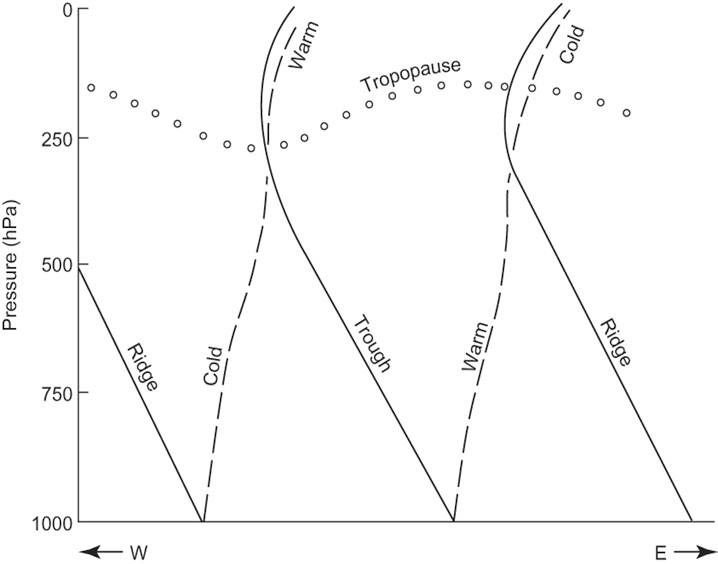
\includegraphics[width=0.4\textwidth]{images/ch05/p15_img01.jpeg}
  \caption{Vertical cross-section of a developing baroclinic wave.
    Solid lines denote geopotential height contours (ridges and troughs);
    dashed lines denote isotherms.  Note the characteristic
    \textgr{westward tilt with height} of the trough and ridge axes:
    warm air rises ahead of the trough while cold air sinks behind it,
    converting mean-flow APE to eddy KE.
    \hisu{경압파의 연직 단면.  기압골/기압능 축이 고도에 따라 서쪽으로 기울어져 있어
          따뜻한 공기는 상승, 차가운 공기는 하강 --- APE에서 KE로의 에너지 변환이 일어남.}}
  \label{fig:baroclinic-westward-tilt}
\end{figure}

\begin{hisublock}
\textbf{참고 문헌 가이드:}
\begin{itemize}
  \item Marshall \& Plumb (2008), \textit{Atmosphere, Ocean, and Climate Dynamics}, Ch.~8.2.2 (pp.~145--148, PDF pp.~166--169) -- baroclinic instability의 기본 메커니즘과 GFD Lab XI 실험
  \item Marshall \& Plumb (2008), Ch.~8.3 (pp.~149--153, PDF pp.~170--174) -- thermal wind equation의 energetics와 APE 방출
  \item Holton \& Hakim Ch.~7 -- 경압 불안정의 수학적 이론 (Eady, Charney problem)
\end{itemize}
\end{hisublock}

% --------------------------------------------------------------------------
\subsection{Baroclinic Wave Lifecycle}
% --------------------------------------------------------------------------

전형적인 baroclinic wave의 lifecycle은 세 단계를 거친다:

\begin{enumerate}
  \item \textgr{Incipient developing stage}: A small-amplitude perturbation
        with a westward tilt with height begins to grow by extracting APE
        from the mean meridional temperature gradient.
  \item \textgr{Rapid development stage}: The disturbance amplifies rapidly.
        Upper-level PV anomalies and surface temperature anomalies interact
        cooperatively, reinforcing each other (mutual amplification).
  \item \textgr{Occlusion stage}: The wave matures, the surface fronts wrap
        around the low centre, the warm sector narrows, and the system begins
        to decay as the westward tilt is lost and energy conversion ceases.
\end{enumerate}

\hisu{경압파 생애주기: 발달 초기 → 급속 발달 → 폐색.  서쪽 기울기가 사라지면 에너지 변환이 멈추고 파동이 소멸.}

\begin{figure}[htbp]
  \centering
  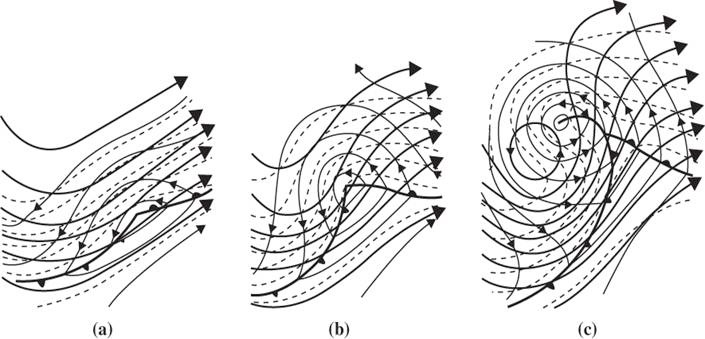
\includegraphics[width=0.7\textwidth]{images/ch05/p17_img01.jpeg}
  \caption{Schematic of baroclinic wave lifecycle at the surface:
    (a)~incipient developing stage with small-amplitude perturbations,
    (b)~rapid development stage with amplifying warm and cold fronts, and
    (c)~occlusion stage where the warm sector narrows and the system
    begins to decay.  Solid lines: isobars; dashed lines: fronts;
    arrows: surface wind.
    \hisu{경압파 생애주기 모식도: (a)~발달 초기, (b)~급속 발달기 (전선 강화),
          (c)~폐색기 (온난역 축소, 시스템 소멸).}}
  \label{fig:baroclinic-lifecycle}
\end{figure}

\begin{figure}[htbp]
  \centering
  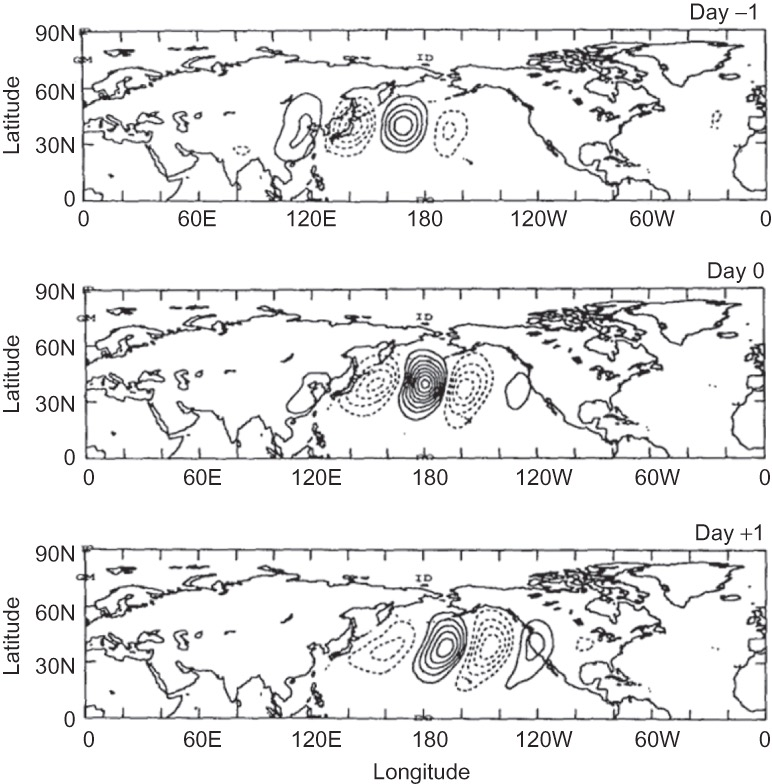
\includegraphics[width=0.45\textwidth]{images/ch05/p13_img01.jpeg}\hfill
  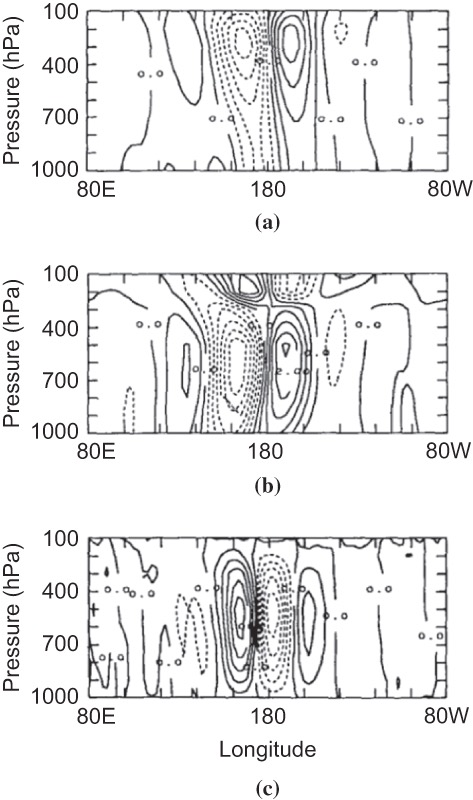
\includegraphics[width=0.45\textwidth]{images/ch05/p13_img02.jpeg}
  \caption{Observed storm-track disturbance composite.
    Left: 500\,hPa geopotential height anomaly at Day~$-1$, Day~0, and
    Day~$+1$, showing eastward propagation of the upper-level wave.
    Right: longitude--pressure cross-sections at the corresponding times,
    illustrating the westward tilt with height during the developing stage
    and the progressive vertical alignment toward occlusion.
    \hisu{관측 storm track 교란 합성장.  왼쪽: 500\,hPa 고도 이상 (동진하는 상층파).
          오른쪽: 경도--기압 단면 (발달기의 서쪽 기울기와 폐색기의 연직 정렬).}}
  \label{fig:storm-track-composite}
\end{figure}

\begin{hisublock}
\textbf{참고 문헌 가이드:}
\begin{itemize}
  \item Hartmann (1994), \textit{Global Physical Climatology}, Ch.~6.3 (book pp.~138--149; 본 PDF에는 목차만 수록) -- 중위도 에디의 meridional energy transport와 lifecycle
  \item Peixoto \& Oort (1992), \textit{Physics of Climate}, Ch.~14.5 (book pp.~385--392; 본 PDF에는 목차만 수록) -- EP flux와 zonal-mean state의 유지
\end{itemize}
\end{hisublock}


% =============================================================================
\section{\texorpdfstring{Derivation of QG Equations (\(z\)-coordinate)}{Derivation of QG Equations (z-coordinate)}}\label{sec:qg-z}
% =============================================================================

Quasi-geostrophic (QG) equations는 중위도 기상 시스템을 이해하기 위한
가장 중요한 역학적 framework이다.
이 방정식은 \textgr{Rossby number의 작음}, $\mathrm{Ro} = U/(fL) \sim 0.1$을 체계적으로 이용하여,
빠른 inertia-gravity waves를 걸러내고 온대 대기를 지배하는 느린 balanced motions만을
보존하도록 유도된다.

\hisu{QG 방정식 = Rossby 수가 작을 때 ($\mathrm{Ro}\sim 0.1$), 느린 균형 운동만을 기술하는 근사 체계}

% --------------------------------------------------------------------------
\subsection{Boussinesq Approximation}\label{subsec:boussinesq}
% --------------------------------------------------------------------------

\begin{definition}[Boussinesq Approximation]
In the Boussinesq approximation, density variations are neglected everywhere
except in the \textgr{buoyancy term} of the vertical momentum equation.
A constant reference density $\rho_0$ replaces $\rho$ in all other terms.
The governing equations become:
\begin{align}
  \frac{Du}{Dt} &= -\frac{1}{\rho_0}\frac{\partial p}{\partial x}
                    + fv + F_x, \label{eq:bous-x}\\[4pt]
  \frac{Dv}{Dt} &= -\frac{1}{\rho_0}\frac{\partial p}{\partial y}
                    - fu + F_y, \label{eq:bous-y}\\[4pt]
  \frac{Dw}{Dt} &= -\frac{1}{\rho_0}\frac{\partial p}{\partial z}
                    - g + g\frac{\theta}{\theta_0} + F_z, \label{eq:bous-z}
\end{align}
where $\theta_{\mathrm{tot}}(x,y,z,t) = \theta_0(z) + \theta(x,y,z,t)$ is the
total potential temperature decomposed into a horizontally uniform reference
profile $\theta_0(z)$ and a perturbation $\theta$.
\hisu{밀도 변화가 작으므로 부력항을 제외하고는 상수 $\rho_0$로 근사}
\end{definition}

\begin{hisublock}
Boussinesq 근사의 핵심 아이디어:
\begin{itemize}
  \item 대기에서 밀도 변동 $\rho'/\rho_0 \sim 1\%$이므로, 관성항에서의 밀도 차이는 무시 가능
  \item 그러나 중력과 결합하면 $g\rho'/\rho_0$는 작지 않으므로 부력항에서는 반드시 유지
  \item 연속 방정식이 $\nabla\cdot\mathbf{V} + \partial w/\partial z = 0$ (비압축성)으로 단순화
\end{itemize}
\end{hisublock}

\noindent
Boussinesq approximation 하에서 \textgr{mass continuity equation}은
incompressible form으로 단순화된다:
\begin{equation}\label{eq:bous-cont}
  \frac{\partial u}{\partial x}
  + \frac{\partial v}{\partial y}
  + \frac{\partial w}{\partial z} = 0.
\end{equation}

% --------------------------------------------------------------------------
\subsection{Geostrophic Relations}\label{subsec:geostrophic}
% --------------------------------------------------------------------------

Rossby number의 leading order에서 수평 운동량 방정식
\eqref{eq:bous-x}--\eqref{eq:bous-y}는 \textgr{geostrophic balance}로 환원된다:

\begin{equation}\label{eq:geowind}
  u_g = -\frac{1}{\rho_0 f}\frac{\partial p}{\partial y},
  \qquad
  v_g = +\frac{1}{\rho_0 f}\frac{\partial p}{\partial x}.
\end{equation}

\noindent
In vector form:
\begin{equation}\label{eq:geowind-vec}
  \mathbf{V}_g = \frac{1}{\rho_0 f}\,\hat{k}\times\nabla p.
\end{equation}

\begin{remark}[Properties of Geostrophic Wind]
\begin{itemize}
  \item $\mathbf{V}_g$ is \textgr{non-divergent}:
        $\nabla\cdot\mathbf{V}_g = 0$ (on an $f$-plane).
  \item $\mathbf{V}_g$ is parallel to isobars, with low pressure to the left
        in the Northern Hemisphere.
  \item The geostrophic wind completely determines the horizontal pressure field
        (and vice versa) at any given level.
\end{itemize}
\end{remark}

\subsubsection{Geostrophic Vorticity}

\textgr{Geostrophic vorticity}의 연직 성분은 $\mathbf{V}_g$로부터 다음과 같이 얻어진다:
\begin{equation}\label{eq:geovort}
  \zeta_g
  = \frac{\partial v_g}{\partial x} - \frac{\partial u_g}{\partial y}
  = \frac{1}{\rho_0 f}\left(
      \frac{\partial^2 p}{\partial x^2}
    + \frac{\partial^2 p}{\partial y^2}
  \right)
  = \frac{1}{\rho_0 f}\nabla^2 p.
\end{equation}

\hisu{지균 소용돌이도는 압력장의 수평 라플라시안에 비례 — 압력장만으로 완전히 결정됨}

\subsubsection{QG Material Derivative}

QG framework에서 material derivative는 수평 이류에
\emph{geostrophic wind만}을 사용하여 평가된다:
\begin{equation}\label{eq:qg-ddt}
  \frac{d}{dt}
  \equiv \frac{\partial}{\partial t}
       + u_g\frac{\partial}{\partial x}
       + v_g\frac{\partial}{\partial y}.
\end{equation}

\begin{hisublock}
QG material derivative에서 주의할 점:
\begin{itemize}
  \item 수평 이류는 \textbf{지균풍}만 사용 (비지균풍에 의한 이류는 $O(\mathrm{Ro})$ 작음)
  \item 연직 이류 $w\,\partial/\partial z$는 포함되지 \textbf{않음}
        (열역학 방정식에서만 연직 운동이 나타남)
  \item 이것이 QG 방정식이 수학적으로 다루기 쉬운 핵심 이유
\end{itemize}
\end{hisublock}

% --------------------------------------------------------------------------
\subsection{Hydrostatic Balance and Thermal Wind}\label{subsec:thermal-wind}
% --------------------------------------------------------------------------

연직 운동량 방정식 \eqref{eq:bous-z}에 hydrostatic approximation과
Boussinesq approximation을 적용하면 \textgr{perturbation hydrostatic
relation}을 얻는다:
\begin{equation}\label{eq:hydro-pert}
  \frac{\partial p}{\partial z} = \frac{\rho_0\,g}{\theta_0}\,\theta.
\end{equation}

\noindent
Geostrophic relations \eqref{eq:geowind}을 $z$에 대해 미분하고
\eqref{eq:hydro-pert}를 대입하면
\textgr{thermal wind relation}을 얻는다:

\begin{equation}\label{eq:thermal-wind-ch05}
  \frac{\partial \mathbf{V}_g}{\partial z}
  = \frac{g}{f\,\theta_0}\,\hat{k}\times\nabla\theta.
\end{equation}

\noindent
In component form:
\begin{equation}\label{eq:thermal-wind-comp}
  \frac{\partial u_g}{\partial z}
  = -\frac{g}{f\,\theta_0}\frac{\partial\theta}{\partial y},
  \qquad
  \frac{\partial v_g}{\partial z}
  = +\frac{g}{f\,\theta_0}\frac{\partial\theta}{\partial x}.
\end{equation}

\begin{hisublock}
열역풍 관계의 물리적 의미:
\begin{itemize}
  \item 연직 바람 시어는 수평 온도 경도에 비례
  \item 남쪽이 따뜻하면 ($\partial\theta/\partial y < 0$) → $\partial u_g/\partial z > 0$ → 상층으로 갈수록 서풍 증가
  \item 이것이 중위도 제트가 존재하는 이유: 적도-극 온도차가 상층 서풍 시어를 생성
\end{itemize}
\end{hisublock}

% --------------------------------------------------------------------------
\subsection{Thermodynamic Energy Equation}\label{subsec:thermo-z}
% --------------------------------------------------------------------------

QG framework에서 perturbation potential temperature $\theta$에 대한 thermodynamic equation은
다음과 같다:
\begin{equation}\label{eq:thermo-qg-z}
  \frac{d\theta}{dt} = -w\,\frac{d\theta_0}{dz},
\end{equation}

\noindent
여기서 좌변은 QG material derivative \eqref{eq:qg-ddt}를 사용하며,
우변은 안정 성층 배경에서 연직 운동에 의한 adiabatic cooling/heating을 나타낸다.

\begin{definition}[Brunt--V\"{a}is\"{a}l\"{a} Frequency]
The \emph{Brunt--V\"{a}is\"{a}l\"{a} frequency} $N$ measures the static stability
of the background stratification:
\begin{equation}\label{eq:BV-freq}
  N = \left[\frac{g}{\theta_0}\frac{d\theta_0}{dz}\right]^{1/2}.
\end{equation}
Typical tropospheric values: $N \approx 0.01$\,s$^{-1}$.
For a stably stratified atmosphere, $d\theta_0/dz > 0$ so $N^2 > 0$.
\hisu{$N^2>0$이면 안정, $N^2<0$이면 정적 불안정 (대류 발생)}
\end{definition}

\noindent
\eqref{eq:BV-freq}를 이용하면 thermodynamic equation \eqref{eq:thermo-qg-z}를
다음과 같이 쓸 수 있다:
\begin{equation}\label{eq:thermo-qg-z-N}
  \frac{d\theta}{dt} = -\frac{\theta_0 N^2}{g}\,w.
\end{equation}

% --------------------------------------------------------------------------
\subsection{Gradient and Laplacian --- Geometric Intuition}\label{subsec:grad-lap}
% --------------------------------------------------------------------------

QG theory에서 반복적으로 나타나는 두 미분 연산자는
주의 깊은 기하학적 해석이 필요하다.

\subsubsection{The Gradient}

Gradient $\nabla\Phi$는 scalar field $\Phi$의 \textgr{steepest ascent} 방향을 가리키며,
그 크기는 최대 변화율과 같다.  $\Phi$의 등고선은 $\nabla\Phi$에 수직이다.

\begin{figure}[htbp]
  \centering
  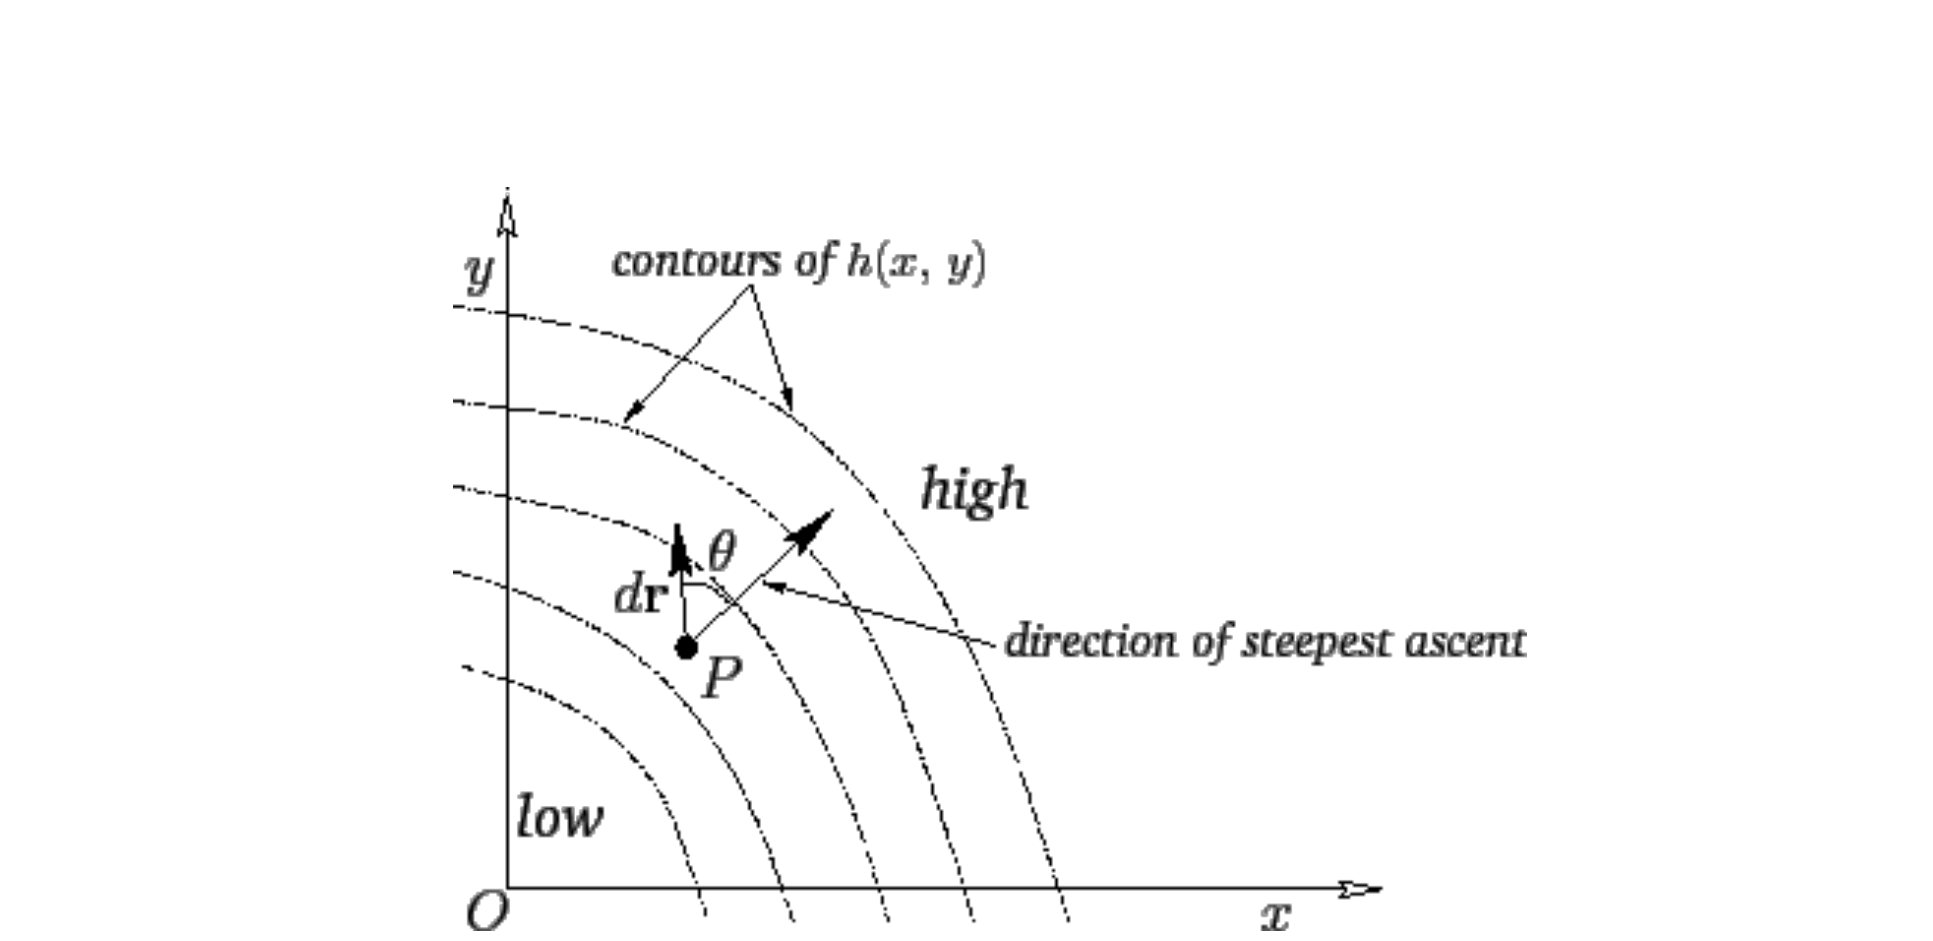
\includegraphics[width=0.45\textwidth]{images/ch05/p30_img01.png}\hfill
  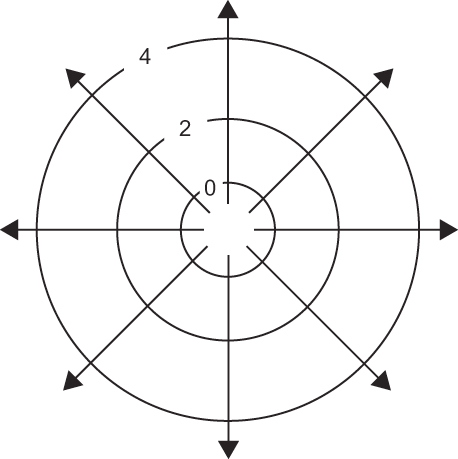
\includegraphics[width=0.40\textwidth]{images/ch05/p29_img01.png}
  \caption{Left: Contours of a scalar field $h(x,y)$ with the gradient
    vector $\nabla h$ pointing in the direction of steepest ascent,
    perpendicular to isolines.
    Right: Illustration of gradient vectors radiating outward from a
    local minimum, showing the relationship between contour spacing and
    gradient magnitude.
    \hisu{왼쪽: 등고선에 수직인 경도(gradient) 벡터 --- 최대 상승 방향을 가리킨다.
          오른쪽: 극소점 주변의 경도 벡터 분포.}}
  \label{fig:gradient-illustration}
\end{figure}

\subsubsection{The Laplacian}

Laplacian $\nabla^2\Phi$는 한 점에서의 $\Phi$ 값이 작은 이웃 영역의
평균으로부터 얼마나 벗어나는지를 측정한다:

\begin{remark}[Sign Convention of the Laplacian]
\begin{itemize}
  \item $\nabla^2\Phi > 0$ at a \textgr{local minimum} of $\Phi$:
        the value at the point is \emph{less than} the neighbourhood average.
  \item $\nabla^2\Phi < 0$ at a \textgr{local maximum} of $\Phi$:
        the value at the point is \emph{greater than} the neighbourhood average.
\end{itemize}
\end{remark}

\hisu{라플라시안이 양수 = 극소점 (주변보다 값이 작음), 음수 = 극대점 (주변보다 값이 큼)}

\begin{hisublock}
QG 이론에서의 응용:
\begin{itemize}
  \item $\nabla^2 p > 0$ → 기압 극소 → $\zeta_g > 0$ → 저기압성 소용돌이도
  \item $\nabla^2 p < 0$ → 기압 극대 → $\zeta_g < 0$ → 고기압성 소용돌이도
\end{itemize}
따라서 저기압 중심에서는 항상 양의 (저기압성) 소용돌이도를 갖는다.
\end{hisublock}

\begin{hisublock}
\textbf{참고 문헌 가이드:}
\begin{itemize}
  \item Holton \& Hakim Ch.~6.2--6.3 -- QG equations의 체계적 유도 ($z$-좌표)
  \item Vallis, \textit{Atmospheric and Oceanic Fluid Dynamics}, Ch.~5.1--5.3 -- Boussinesq QG framework
  \item Marshall \& Plumb (2008), \textit{Atmosphere, Ocean, and Climate Dynamics}, Ch.~8.2.2 (pp.~145--148, PDF pp.~166--169) -- geostrophic balance와 thermal wind의 물리적 해석
\end{itemize}
\end{hisublock}


% =============================================================================
\section{QG Potential Vorticity}\label{sec:qgpv}
% =============================================================================

\textbf{Potential vorticity} (PV) 개념은 geophysical fluid dynamics에서
가장 강력한 아이디어이다.  QG framework에서 PV는
특히 우아하고 유용한 형태를 취한다.

% --------------------------------------------------------------------------
\subsection{From Ertel PV to QG PV}\label{subsec:ertel-to-qg}
% --------------------------------------------------------------------------

\subsubsection{Ertel PV under the Boussinesq Approximation}

Boussinesq 유체에 대한 정확한 (Ertel) potential vorticity는 다음과 같다:
\begin{equation}\label{eq:ertel}
  \Pi = \frac{\boldsymbol{\omega}_a \cdot \nabla\theta_{\mathrm{tot}}}{\rho_0},
\end{equation}
where $\boldsymbol{\omega}_a = \nabla\times\mathbf{V} + f\hat{k}$ is the
absolute vorticity vector이다.  Adiabatic, frictionless flow에서 Ertel PV는
materially conserved된다:
\begin{equation}\label{eq:ertel-conserve}
  \frac{D\Pi}{Dt} = 0.
\end{equation}

\subsubsection{QG Scaling of Ertel PV}

$\theta_{\mathrm{tot}} = \theta_0(z) + \theta(x,y,z,t)$와
$\boldsymbol{\omega}_a = (\xi, \eta, \zeta + f)$ (여기서 $(\xi,\eta)$는
수평 vorticity 성분)를 전개하면:
\begin{equation}\label{eq:ertel-expand}
  \Pi = \frac{1}{\rho_0}\left[
    \xi\frac{\partial\theta}{\partial x}
    + \eta\frac{\partial\theta}{\partial y}
    + (\zeta + f)\left(\frac{d\theta_0}{dz} + \frac{\partial\theta}{\partial z}\right)
  \right].
\end{equation}

\noindent
QG scaling ($\mathrm{Ro} \ll 1$) 하에서:
\begin{enumerate}
  \item The horizontal vorticity terms $\xi\,\partial\theta/\partial x$ and
        $\eta\,\partial\theta/\partial y$ are $O(\mathrm{Ro}^2)$ smaller than the
        vertical terms, so we neglect them.
  \item In the vertical term, $\zeta\,\partial\theta/\partial z$ is
        $O(\mathrm{Ro})$ compared to $f\,d\theta_0/dz$, so we keep only
        the leading-order contributions.
  \item We retain $\zeta_g$ (not the full $\zeta$) and replace $\zeta$ by $\zeta_g$.
\end{enumerate}

\noindent
주의 깊은 차수 정리 후, Ertel PV의 QG-relevant 부분은 다음으로 환원된다:
\begin{equation}\label{eq:ertel-qg-reduce}
  \Pi \approx \frac{1}{\rho_0}\left[
    (\zeta_g + f)\frac{d\theta_0}{dz}
    + f\frac{\partial\theta}{\partial z}
  \right].
\end{equation}

\noindent
기준 안정도 $(1/\rho_0)\,d\theta_0/dz$로 나누고 정리하면,
\textgr{QG potential vorticity}를 다음과 같이 정의한다:

\begin{definition}[QG Potential Vorticity, $z$-coordinate]
\begin{equation}\label{eq:qgpv-z}
  \boxed{
  Q = (\zeta_g + f) + f\,\frac{\partial}{\partial z}
      \left(\frac{\theta}{\partial\theta_0/\partial z}\right).
  }
\end{equation}
The three terms represent:
\begin{enumerate}
  \item $\zeta_g$: relative (geostrophic) vorticity
  \item $f$: planetary vorticity
  \item $f\,\dfrac{\partial}{\partial z}\!\left(\dfrac{\theta}
        {\partial\theta_0/\partial z}\right)$:
        \textgr{stretching vorticity} (vertical redistribution of stability)
\end{enumerate}
\end{definition}

\begin{hisublock}
QG PV의 세 가지 구성 요소:
\begin{enumerate}
  \item \textbf{상대 소용돌이도} $\zeta_g$: 유체 자체의 회전
  \item \textbf{행성 소용돌이도} $f$: 지구 자전에 의한 기여
  \item \textbf{신축 소용돌이도}: 연직 안정도의 변형에 의한 소용돌이도
\end{enumerate}
Ertel PV는 소용돌이도와 안정도의 \textbf{곱}이지만,
QG PV는 \textbf{합}으로 정의됨.
소용돌이도가 증가하면 안정도가 감소해야 PV가 보존된다.
\end{hisublock}

% --------------------------------------------------------------------------
\subsection{QG PV Conservation}\label{subsec:qgpv-conserve}
% --------------------------------------------------------------------------

QG theory의 가장 근본적인 결과는 $Q$가 \emph{geostrophic flow}를 따라
materially conserved된다는 것이다:

\begin{theorem}[Conservation of QG PV]
For adiabatic, frictionless, quasi-geostrophic flow:
\begin{equation}\label{eq:qgpv-conserve}
  \boxed{
  \frac{dQ}{dt}
  = \left(\frac{\partial}{\partial t}
    + u_g\frac{\partial}{\partial x}
    + v_g\frac{\partial}{\partial y}\right) Q = 0.
  }
\end{equation}
\end{theorem}

\hisu{QG PV는 지균류를 따라 보존된다 --- QG 이론의 핵심 결과!  이 하나의 방정식이 QG 역학 전체를 지배한다.}

\begin{proof}
We derive this from the QG vorticity and thermodynamic equations.

\textit{Step 1.}  The QG vorticity equation (derived in Sec.~\ref{subsec:qg-vort-eq})
gives:
\[
  \frac{d}{dt}(\zeta_g + f) = f\frac{\partial w}{\partial z}.
\]

\textit{Step 2.}  The QG thermodynamic equation \eqref{eq:thermo-qg-z} gives:
\[
  \frac{d\theta}{dt} = -w\frac{d\theta_0}{dz}.
\]
Dividing by $d\theta_0/dz$ and taking $\partial/\partial z$:
\[
  \frac{\partial}{\partial z}\!\left(\frac{1}{d\theta_0/dz}\frac{d\theta}{dt}\right)
  = -\frac{\partial w}{\partial z}.
\]
Since $d\theta_0/dz$ depends only on $z$ (not on $x,y,t$), we can move the
material derivative outside:
\[
  \frac{d}{dt}\frac{\partial}{\partial z}
  \!\left(\frac{\theta}{d\theta_0/dz}\right) = -\frac{\partial w}{\partial z}.
\]
Multiplying by $f$:
\[
  f\frac{d}{dt}\frac{\partial}{\partial z}
  \!\left(\frac{\theta}{d\theta_0/dz}\right) = -f\frac{\partial w}{\partial z}.
\]

\textit{Step 3.}  Adding the vorticity equation (Step~1) and the rearranged
thermodynamic equation (Step~2):
\[
  \frac{d}{dt}\!\left[
    (\zeta_g + f) + f\frac{\partial}{\partial z}
    \!\left(\frac{\theta}{d\theta_0/dz}\right)
  \right] = 0,
\]
which is precisely $dQ/dt = 0$.
\end{proof}

% --------------------------------------------------------------------------
\subsection{QG Vorticity Equation}\label{subsec:qg-vort-eq}
% --------------------------------------------------------------------------

QG vorticity equation은 수평 운동량 방정식에서
$\partial v_g/\partial x - \partial u_g/\partial y$를 취하고 QG scaling을
적용하여 얻는다.  그 결과는 다음과 같다:

\begin{equation}\label{eq:qg-vort-z}
  \boxed{
  \frac{d}{dt}(\zeta_g + f) = f\,\frac{\partial w}{\partial z}.
  }
\end{equation}

\begin{remark}[Physical Interpretation]
\begin{itemize}
  \item 좌변: geostrophic flow를 따른 \textgr{absolute geostrophic vorticity}의 변화율.
  \item 우변: planetary vorticity tubes의 \textgr{stretching/compression}에 의한
        vorticity 생성.
  \item $\partial w/\partial z > 0$ (stretching)이면: 기둥이 더 높고 가늘어짐 → spin-up (cyclonic vorticity 증가).
  \item $\partial w/\partial z < 0$ (compression)이면: 기둥이 더 낮고 넓어짐 → spin-down (anticyclonic vorticity 증가).
\end{itemize}
\end{remark}

\hisu{절대 소용돌이도의 변화 = 행성 소용돌이 관(vortex tube)의 신축(stretching)에 의한 것}

\begin{hisublock}
유도 과정의 핵심:
\begin{enumerate}
  \item 수평 운동 방정식에서 $\partial/\partial x(\text{v-eq}) - \partial/\partial y(\text{u-eq})$ 취함
  \item 지균풍이 비발산이므로 $\nabla\cdot\mathbf{V}_g = 0$
  \item 비지균풍의 수평 발산 $\partial u_a/\partial x + \partial v_a/\partial y$가 연속 방정식으로부터
        $-\partial w/\partial z$와 연결
  \item 결과적으로 소용돌이도 변화가 연직 운동의 수렴/발산으로 결정됨
\end{enumerate}
\end{hisublock}

% --------------------------------------------------------------------------
\subsection{QG Mass Continuity}\label{subsec:qg-cont}
% --------------------------------------------------------------------------

전체 수평 바람을
$\mathbf{V} = \mathbf{V}_g + \mathbf{V}_a$로 분해한다. 여기서 $\mathbf{V}_a$는
\textgr{ageostrophic wind}이다.  $f$-plane에서 $\nabla\cdot\mathbf{V}_g = 0$이므로,
Boussinesq continuity equation \eqref{eq:bous-cont}은 다음이 된다:

\begin{equation}\label{eq:qg-cont}
  \frac{\partial u_a}{\partial x}
  + \frac{\partial v_a}{\partial y}
  + \frac{\partial w}{\partial z} = 0.
\end{equation}

\hisu{지균풍은 비발산이므로, 수평 발산은 전적으로 비지균풍에 의한 것이다.  이 비지균 발산이 연직 운동을 구동한다.}

% --------------------------------------------------------------------------
\subsection{QG PV in Terms of Pressure Alone}\label{subsec:qgpv-pressure}
% --------------------------------------------------------------------------

QG system의 놀라운 특징은 모든 역학적 물리량을
\textgr{단일 변수}인 pressure perturbation $p$로 표현할 수 있다는 것이다.
$\zeta_g = (1/\rho_0 f)\nabla^2 p$와
$\theta = (\theta_0/\rho_0 g)\,\partial p/\partial z$ (hydrostatic
relation \eqref{eq:hydro-pert}로부터)를 \eqref{eq:qgpv-z}에 대입하면:

\begin{equation}\label{eq:qgpv-p-only}
  \boxed{
  f\,(Q - f) = \frac{1}{\rho_0}\nabla^2 p
    + \frac{1}{\rho_0}\frac{\partial}{\partial z}
      \!\left(\frac{f^2}{N^2}\frac{\partial p}{\partial z}\right)
    \equiv Lp.
  }
\end{equation}

\noindent
연산자 $L$은 3차원 elliptic operator (``invertibility operator'')로서,
pressure field를 PV distribution으로 mapping한다.

\hisu{QG PV는 압력장 하나로 완전히 결정 --- 매우 강력한 결과!}

\begin{hisublock}
이것이 강력한 이유: PV 분포 $Q(x,y,z)$를 알면, 적절한 경계 조건과 함께
$L p = f(Q - f)$를 풀어서 $p$를 구하고, $p$로부터 바람, 온도, 소용돌이도를
모두 진단(diagnose)할 수 있다.  이것이 \textbf{PV 역전(inversion)} 원리이다:
\[
  Q \xrightarrow{\text{inversion}} p
  \xrightarrow{\text{geostrophic}} \mathbf{V}_g, \;\theta, \;\zeta_g.
\]
\end{hisublock}

\begin{hisublock}
\textbf{참고 문헌 가이드:}
\begin{itemize}
  \item Holton \& Hakim Ch.~6.3 -- QG PV의 유도와 보존 법칙
  \item Vallis Ch.~5.3--5.4 -- Ertel PV에서 QG PV로의 체계적 유도
  \item Hoskins, McIntyre, \& Robertson (1985) -- PV inversion의 개념과 응용
\end{itemize}
\end{hisublock}


% =============================================================================
\section{QG Height Tendency Equation}\label{sec:qg-height-tendency}
% =============================================================================

QG height tendency equation은 현재 바람과 온도의 분포가 주어졌을 때
pressure field가 시간에 따라 어떻게 진화하는지를 예측하는 \textgr{prognostic equation}이다.
이는 synoptic weather forecasting의 이론적 기초이다.

% --------------------------------------------------------------------------
\subsection{Derivation}\label{subsec:height-tendency-derive}
% --------------------------------------------------------------------------

QG PV conservation \eqref{eq:qgpv-conserve}과
invertibility relation \eqref{eq:qgpv-p-only}에서 출발한다.

\textit{Step 1.}  From $dQ/dt = 0$:
\begin{equation}\label{eq:ht-step1}
  \frac{\partial Q}{\partial t} = -\mathbf{V}_g\cdot\nabla Q.
\end{equation}

\textit{Step 2.}  Noting that $f$ is time-independent on a $\beta$-plane
(i.e.\ $\partial f/\partial t = 0$), we have
$\partial Q/\partial t = (1/f)\,\partial(Lp)/\partial t$,
and $\nabla Q$ includes $\nabla f = \beta\hat{j}$ plus eddy PV gradients.
Combining:
\begin{equation}\label{eq:ht-step2}
  L\frac{\partial p}{\partial t} = -f\,\mathbf{V}_g\cdot\nabla Q.
\end{equation}

\textit{Step 3.}  Expanding $fQ = f(\zeta_g + f) + f^2\,\partial_z(\theta/(d\theta_0/dz))$
and using the identity $\mathbf{V}_g\cdot\nabla f = \beta v_g$:

\begin{equation}\label{eq:height-tendency-z}
  \boxed{
  L\frac{\partial p}{\partial t}
  = -\mathbf{V}_g\cdot\nabla(f\zeta_g)
    + f^2\frac{\partial}{\partial z}
      \!\left[\frac{\mathbf{V}_g\cdot\nabla\theta}
              {\partial\theta_0/\partial z}\right].
  }
\end{equation}

% --------------------------------------------------------------------------
\subsection{Physical Interpretation}\label{subsec:height-tendency-phys}
% --------------------------------------------------------------------------

\eqref{eq:height-tendency-z}의 우변에 있는 두 forcing terms은
명확한 물리적 해석을 갖는다:

\begin{remark}[Height Tendency Forcing Terms]
\begin{enumerate}
  \item \textgr{Vorticity advection} $(-\mathbf{V}_g\cdot\nabla(f\zeta_g))$:
        Advection of absolute vorticity by the geostrophic wind.
        \begin{itemize}
          \item Cyclonic vorticity advection ($-\mathbf{V}_g\cdot\nabla\zeta_g > 0$)
                → $L(\partial p/\partial t) > 0$ → since $L$ reverses the sign
                (like $\nabla^2$), this implies \textgr{pressure falls}
                → low deepens.
          \item Anticyclonic vorticity advection → pressure rises → high builds.
        \end{itemize}
  \item \textgr{Differential temperature advection}:
        Upward increase of warm advection
        ($\partial/\partial z[{-\mathbf{V}_g\cdot\nabla(-\theta)}] > 0$)
        → pressure falls → low deepens.
        \begin{itemize}
          \item Warm advection increasing with height destabilises the column,
                requiring convergence at low levels, which spins up a surface low.
          \item Cold advection increasing with height stabilises the column,
                producing divergence at low levels and building a surface high.
        \end{itemize}
\end{enumerate}
\end{remark}

\hisu{저기압 발달 조건: 저기압성 소용돌이도 이류 + 온난 이류의 상향 증가.  이 두 효과가 같은 위치에서 협력하면 급속한 저기압 발달 (폭풍 발달)이 일어남!}

\begin{hisublock}
실제 일기예보에서의 응용:
\begin{itemize}
  \item 500\,hPa 절대 소용돌이도 이류(AVA)가 양이면 → 지상 기압 하강 예상
  \item 하층에서 온난 이류 + 상층에서 더 강한 온난 이류 → 기압 하강 촉진
  \item 두 효과가 겹치는 곳에서 explosive cyclogenesis 가능
\end{itemize}
\end{hisublock}

\begin{hisublock}
\textbf{참고 문헌 가이드:}
\begin{itemize}
  \item Holton \& Hakim Ch.~6.4 -- QG height tendency equation의 유도와 일기예보 응용
  \item Bluestein, \textit{Synoptic-Dynamic Meteorology}, Vol.~II -- vorticity advection과 thermal advection의 실제 일기도 분석
\end{itemize}
\end{hisublock}


% =============================================================================
\section{QG Vertical Motion Equation}\label{sec:qg-omega-z}
% =============================================================================

대기의 vertical motion은 직접 측정할 수 없으며, 다른 장(field)으로부터
\textgr{진단(diagnosed)}되어야 한다.  QG omega equation은 이를 위한
강력한 도구를 제공한다.

% --------------------------------------------------------------------------
\subsection{Omega Equation ($z$-coordinate)}\label{subsec:omega-eq-z}
% --------------------------------------------------------------------------

Omega equation은 QG vorticity equation \eqref{eq:qg-vort-z}과 QG thermodynamic
equation \eqref{eq:thermo-qg-z} 사이에서 $\partial p/\partial t$를 소거하여
유도된다.

\textit{Step 1.}  Take $\partial/\partial z$ of the vorticity equation:
\[
  \frac{\partial}{\partial z}\!\left[\frac{d}{dt}(\zeta_g + f)\right]
  = f\frac{\partial^2 w}{\partial z^2}.
\]

\textit{Step 2.}  Take $\nabla^2$ of the thermodynamic equation
\eqref{eq:thermo-qg-z}:
\[
  \nabla^2\!\left[\frac{d\theta}{dt}\right]
  = -\frac{d\theta_0}{dz}\,\nabla^2 w.
\]

\textit{Step 3.}  Rearrange and combine (using the thermal wind relation to
convert $\partial\zeta_g/\partial z$ terms into $\nabla\theta$ terms):

\begin{equation}\label{eq:omega-z}
  \boxed{
  \underbrace{
  \left(\nabla^2 + \frac{f^2}{N^2}\frac{\partial^2}{\partial z^2}\right)
  }_{\tilde{L}}\,w
  = \frac{g}{\theta_0 N^2}\nabla^2(-\mathbf{V}_g\cdot\nabla\theta)
    - \frac{f}{N^2}\frac{\partial}{\partial z}(-\mathbf{V}_g\cdot\nabla\zeta_g).
  }
\end{equation}

\begin{remark}[Properties of the Omega Equation]
\begin{itemize}
  \item The operator $\tilde{L}$ is an \textgr{elliptic operator} (like a 3D
        Laplacian, with the vertical stretched by $f/N$).  For an elliptic
        operator, $\tilde{L}w > 0$ implies $w < 0$ locally, and vice versa.
        Therefore the sign of $w$ is \textgr{opposite} to the sign of the
        right-hand side.
  \item The equation is \textgr{diagnostic}: it gives $w$ at any instant from
        the known geostrophic fields, without time integration.
  \item Two forcing terms:
    \begin{enumerate}
      \item Laplacian of temperature advection: warm advection
            ($-\mathbf{V}_g\cdot\nabla\theta > 0$) → $\nabla^2(\text{warm adv.}) > 0$
            at the advection maximum → upward motion.
      \item Differential vorticity advection: cyclonic vorticity advection
            increasing with height → upward motion.
    \end{enumerate}
\end{itemize}
\end{remark}

\hisu{오메가 방정식 = 진단 방정식: 수직 운동을 지균풍의 이류 항들로부터 진단한다.  직접 측정 불가능한 $w$를 구하는 유일한 방법!}

% --------------------------------------------------------------------------
\subsection{Application: Cyclogenesis}\label{subsec:cyclogenesis}
% --------------------------------------------------------------------------

QG framework는 중위도 cyclones가 상층과 지표 disturbances의
cooperative interaction을 통해 어떻게 발달하는지에 대한 완전한 그림을 제공한다.

\begin{remark}[QG Mechanism of Cyclogenesis]
\begin{enumerate}
  \item An \textgr{upper-level PV anomaly} (e.g.\ a trough approaching from
        the west) induces cyclonic circulation and ascent downstream and below.
  \item This ascent produces \textgr{low-level convergence}, which spins up a
        surface cyclone (stretching of planetary vorticity tubes:
        $f\,\partial w/\partial z > 0$).
  \item The surface cyclone, with its associated warm and cold fronts, generates
        a \textgr{surface temperature anomaly} (warm air drawn poleward ahead
        of the low).
  \item This surface warm anomaly is equivalent to a positive PV anomaly at
        the surface, which induces \textgr{cyclonic circulation aloft},
        reinforcing the upper-level trough.
  \item The system amplifies as long as the disturbance maintains a
        \textgr{westward tilt with height}, ensuring continued conversion
        of mean-flow APE to eddy KE.
\end{enumerate}
\end{remark}

\begin{hisublock}
경압 저기압 발달의 핵심 메커니즘:
\begin{itemize}
  \item 상층 PV 이상 + 지표 온도 이상 → 상호 강화 (cooperative interaction)
  \item 서쪽으로 기울어진 교란만이 평균류의 PE를 파동의 KE로 전환 가능
  \item 저기압 위의 발산 → 지표 저기압 강화 → 연직 신축이 소용돌이도 증가 유발
  \item 기울기가 사라지면 (연직 정렬) → 에너지 변환 중단 → 폐색 단계
\end{itemize}
\end{hisublock}

\begin{figure}[htbp]
  \centering
  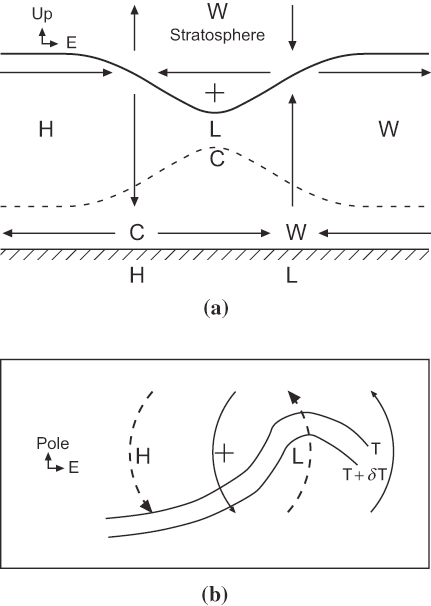
\includegraphics[width=0.65\textwidth]{images/ch05/p58_img01.png}
  \caption{Schematic cross-section of midlatitude cyclogenesis showing the
    interaction between upper-level and surface disturbances.
    (a)~Vertical cross-section: an upper-level trough (with positive PV
    anomaly) induces ascent and low-level convergence, spinning up a
    surface low.  The surface warm anomaly (equivalent to a surface PV
    anomaly) reinforces the upper trough.  Labels H and L denote high
    and low centres; W and C denote warm and cold air.
    (b)~Plan view: the surface cyclone with warm and cold fronts, showing
    warm air advection ahead of the low and cold air intrusion behind.
    \hisu{저기압 발생 모식도.  (a)~연직 단면: 상층 기압골이 하강류·수렴을 유도하여
          지표 저기압 강화.  (b)~평면도: 온난/한랭 전선과 지표 저기압의 배치.}}
  \label{fig:cyclogenesis-schematic}
\end{figure}

\begin{figure}[htbp]
  \centering
  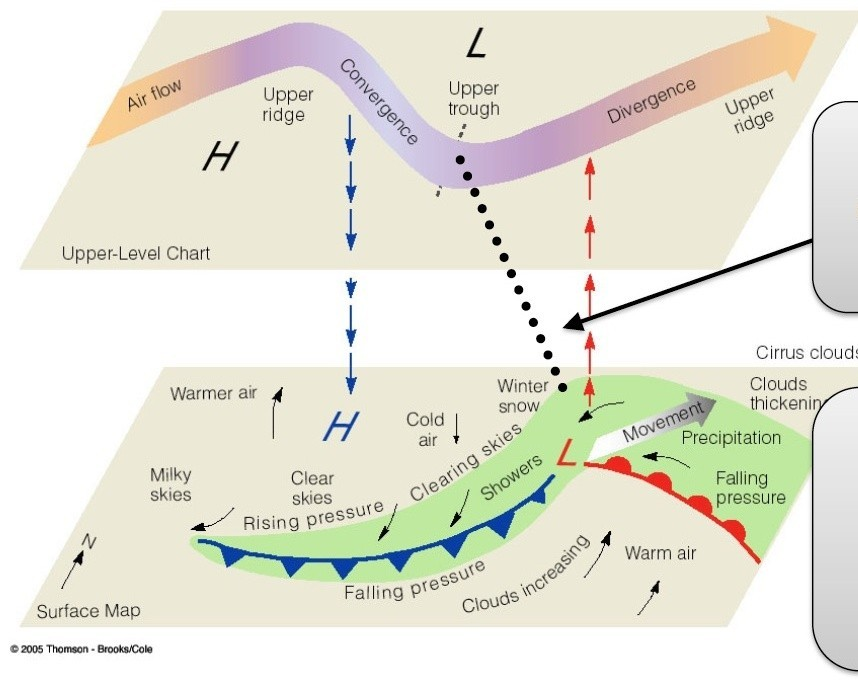
\includegraphics[width=0.8\textwidth]{images/ch05/p111_img01.jpeg}
  \caption{Three-dimensional schematic of the relationship between
    upper-level and surface charts during cyclogenesis.
    Upper panel: 500\,hPa chart with trough (L) and ridge (H) axes;
    convergence upstream and divergence downstream of the upper trough
    are indicated.  Lower panel: surface weather map showing the
    associated cyclone with warm and cold fronts.  The westward tilt
    of the trough axis with height is essential for continued energy
    conversion.
    \hisu{상층 일기도와 지표 일기도의 관계.  상층 기압골의 하류에서 발산 → 지표 저기압 발달.
          서쪽 기울기(tilt with height)가 에너지 변환의 핵심.}}
  \label{fig:upper-surface-cyclogenesis}
\end{figure}

\begin{hisublock}
\textbf{참고 문헌 가이드:}
\begin{itemize}
  \item Holton \& Hakim Ch.~6.4--6.5 -- omega equation 유도와 cyclogenesis에의 응용
  \item Marshall \& Plumb (2008), \textit{Atmosphere, Ocean, and Climate Dynamics}, Ch.~8.3 (pp.~149--153, PDF pp.~170--174) -- APE 방출과 경압 에너지 변환의 energetics
  \item Hartmann (1994), \textit{Global Physical Climatology}, Ch.~6.3 (book pp.~138--149; 본 PDF에는 목차만 수록) -- 에디의 meridional energy transport 역할
\end{itemize}
\end{hisublock}


% =============================================================================
\section{QG Equations in Pressure Coordinates}\label{sec:qg-pressure}
% =============================================================================

실용적 응용---특히 일기예보와 상층 일기도 분석---을 위해
QG equations를 \textgr{pressure coordinates} $(x, y, p, t)$로 정식화하는 것이 편리하다.
여기서 pressure가 height를 대체하여 연직 좌표가 된다.

% --------------------------------------------------------------------------
\subsection{Beta-Plane Approximation}\label{subsec:beta-plane}
% --------------------------------------------------------------------------

\begin{definition}[Beta-Plane Approximation]
The Coriolis parameter is expanded to first order about a reference latitude
$\phi_0$:
\begin{equation}\label{eq:beta-plane}
  f = f_0 + \beta y,
  \qquad
  f_0 = 2\Omega\sin\phi_0,
  \qquad
  \beta = \frac{2\Omega\cos\phi_0}{a},
\end{equation}
where $a$ is the Earth's radius, $\Omega$ its rotation rate, and
$y = a(\phi - \phi_0)$ is the northward distance from the reference latitude.
\end{definition}

\noindent
Scale analysis에 의하면 $\beta$-effect는 $f_0$에 대한 $O(\mathrm{Ro})$
보정임을 확인할 수 있다:
\begin{equation}\label{eq:beta-scaling}
  \frac{\beta L}{f_0} \sim \mathrm{Ro} \sim 0.1.
\end{equation}

\hisu{$\beta$-평면: $f$의 위도 변화를 선형으로 근사.  $\beta L/f_0 \sim \mathrm{Ro}$이므로 $\beta$ 효과는 1차 보정.}

% --------------------------------------------------------------------------
\subsection{QG Momentum Equation (p-coordinate)}\label{subsec:qg-mom-p}
% --------------------------------------------------------------------------

Pressure coordinates에서 geostrophic wind는 다음과 같다:
\begin{equation}\label{eq:geowind-p}
  u_g = -\frac{1}{f_0}\frac{\partial\Phi}{\partial y},
  \qquad
  v_g = +\frac{1}{f_0}\frac{\partial\Phi}{\partial x},
\end{equation}
여기서 $\Phi = gz$는 geopotential이다.  QG momentum equation은 다음과 같다:

\begin{equation}\label{eq:qg-mom-p}
  \boxed{
  \frac{d\mathbf{V}_g}{dt}
  = -f_0\,\hat{k}\times\mathbf{V}_a
    - \beta y\,\hat{k}\times\mathbf{V}_g,
  }
\end{equation}

\noindent
여기서 QG material derivative는
$d/dt = \partial/\partial t + \mathbf{V}_g\cdot\nabla$ (geostrophic wind에 의한
수평 이류만 포함)이다.

\hisu{지균풍의 시간 변화 = 비지균풍에 의한 코리올리 힘 ($-f_0\hat{k}\times\mathbf{V}_a$) + 베타 효과 ($-\beta y\hat{k}\times\mathbf{V}_g$)}

\begin{hisublock}
물리적 의미:
\begin{itemize}
  \item 첫째 항: 비지균풍(ageostrophic wind)에 대한 코리올리 힘이 지균풍을 변화시킴.
        비지균풍이 없으면 지균풍은 변하지 않는다!
  \item 둘째 항: $\beta$ 효과로 인한 보정.  위도에 따라 $f$가 변하므로
        같은 기압 경도라도 다른 위도에서는 다른 지균풍을 줌.
  \item 이 방정식은 ageostrophic motion이 balanced flow의 진화를 구동함을 보여줌.
\end{itemize}
\end{hisublock}

% --------------------------------------------------------------------------
\subsection{QG Thermodynamic Equation (p-coordinate)}\label{subsec:qg-thermo-p}
% --------------------------------------------------------------------------

Pressure coordinates에서의 thermodynamic energy equation은 다음과 같다:
\begin{equation}\label{eq:qg-thermo-p}
  \boxed{
  \left(\frac{\partial}{\partial t}
    + \mathbf{V}_g\cdot\nabla\right)
  \!\left(-\frac{\partial\Phi}{\partial p}\right)
  - \sigma\omega = \frac{\kappa J}{p},
  }
\end{equation}

\noindent
여기서 $-\partial\Phi/\partial p = RT/p = \alpha$는 hydrostatic relation을 통해
온도에 비례하고, $\omega = Dp/Dt$는 pressure-coordinate vertical velocity,
$\sigma(p) = -(\alpha/\theta)\,d\theta/dp > 0$는 \textgr{static
stability parameter}, $J$는 diabatic heating rate, 그리고
$\kappa = R/c_p$이다.

\begin{hisublock}
$p$-좌표에서 열역학 방정식의 각 항:
\begin{itemize}
  \item $(\partial/\partial t + \mathbf{V}_g\cdot\nabla)(-\partial\Phi/\partial p)$:
        두께(온도)의 지균 이류를 포함한 시간 변화
  \item $-\sigma\omega$: 연직 운동에 의한 단열 냉각/가열 ($\omega < 0$이면 상승, 냉각)
  \item $\kappa J/p$: 비단열 가열 (복사, 잠열, 현열 등)
\end{itemize}
\end{hisublock}

% --------------------------------------------------------------------------
\subsection{QG Vorticity Equation (p-coordinate)}\label{subsec:qg-vort-p}
% --------------------------------------------------------------------------

$v_g$-equation에 $(\partial/\partial x)$를, $u_g$-equation에
$(\partial/\partial y)$를 취하고 빼면, continuity equation
$\nabla\cdot\mathbf{V}_a + \partial\omega/\partial p = 0$을 이용하여:

\begin{equation}\label{eq:qg-vort-p}
  \boxed{
  \frac{\partial\zeta_g}{\partial t}
  = -\mathbf{V}_g\cdot\nabla(\zeta_g + f)
    + f_0\frac{\partial\omega}{\partial p}.
  }
\end{equation}

\begin{remark}[Three Mechanisms for Vorticity Change]
\begin{enumerate}
  \item \textgr{Relative vorticity advection}:
        $-\mathbf{V}_g\cdot\nabla\zeta_g$
  \item \textgr{Planetary vorticity advection}:
        $-\mathbf{V}_g\cdot\nabla f = -\beta v_g$
  \item \textgr{Stretching term}:
        $f_0\,\partial\omega/\partial p$
\end{enumerate}
\end{remark}

\begin{hisublock}
각 항의 물리:
\begin{itemize}
  \item 상대 소용돌이도 이류: 소용돌이가 바람에 의해 이동
  \item 행성 소용돌이도 이류: 공기가 북쪽으로 이동하면 ($v_g > 0$) $f$ 증가
        → 상대 소용돌이도 감소 ($\beta$ 효과)
  \item 신축항: $\partial\omega/\partial p > 0$ (하강 약화 또는 상승 강화)
        → 수평 수렴 → 소용돌이도 증가
\end{itemize}
\end{hisublock}

% --------------------------------------------------------------------------
\subsection{Wave Propagation: Short Waves vs.\ Long Waves}
\label{subsec:short-long-waves}
% --------------------------------------------------------------------------

\textgr{Relative vorticity advection}과
\textgr{planetary vorticity advection}이 어떻게 경쟁하는지 이해하기 위해,
간단한 geopotential field를 고려하자:
\begin{equation}\label{eq:wave-geopot}
  \Phi = \Phi_0(p) - f_0\bar{u}\,y + f_0 A\sin(kx)\cos(ly),
\end{equation}
여기서 $\bar{u}$는 상수인 zonal-mean zonal wind이고 $A$는 wave amplitude이다.
\eqref{eq:geowind-p}로부터 geostrophic wind perturbations는:
\[
  u_g' = -\frac{1}{f_0}\frac{\partial\Phi'}{\partial y}
       = Al\sin(kx)\sin(ly),
  \qquad
  v_g' = \frac{1}{f_0}\frac{\partial\Phi'}{\partial x}
       = Ak\cos(kx)\cos(ly).
\]

\noindent
Geostrophic relative vorticity는:
\[
  \zeta_g = \frac{1}{f_0}\nabla^2\Phi'
  = -\frac{(k^2 + l^2)}{f_0}\,f_0 A\sin(kx)\cos(ly)
  = -(k^2 + l^2)\,A\sin(kx)\cos(ly).
\]

\subsubsection{Relative Vorticity Advection}

\[
  -\bar{u}\frac{\partial\zeta_g}{\partial x}
  = \bar{u}(k^2+l^2)\,Ak\cos(kx)\cos(ly).
\]
이는 파동을 \textgr{eastward} ($\bar{u}$의 방향)로 전파시키는 역할을 한다.

\subsubsection{Planetary Vorticity Advection}

\[
  -\beta v_g = -\beta Ak\cos(kx)\cos(ly).
\]
이는 파동을 \textgr{westward} ($\bar{u}$에 반대 방향)로 전파시키는 역할을 한다.

\subsubsection{Ratio of the Two Effects}

Planetary vorticity advection 대 relative vorticity advection의 비는 다음과 같다:
\begin{equation}\label{eq:wave-ratio}
  \boxed{
  \frac{\text{Planetary vorticity advection}}
       {\text{Relative vorticity advection}}
  = \frac{\beta}{\bar{u}(k^2 + l^2)}.
  }
\end{equation}

\begin{remark}[Short Waves vs.\ Long Waves]
\begin{itemize}
  \item \textgr{Short waves} ($k^2 + l^2$ large):
        Relative vorticity advection dominates → net eastward propagation.
        Short waves are swept eastward by the mean flow.
  \item \textgr{Long waves} ($k^2 + l^2$ small):
        Planetary vorticity advection dominates → net westward propagation
        (retrogression).  Very long Rossby waves can propagate westward
        against the mean flow.
  \item \textgr{Stationary waves}: when the two effects exactly cancel,
        i.e.\ $\beta = \bar{u}(k^2 + l^2)$, the wave is stationary.
        The stationary wavenumber is
        $K_s = \sqrt{\beta/\bar{u}}$.
\end{itemize}
\end{remark}

\hisu{단파: 상대 소용돌이도 이류 우세 → 동진.  장파: 행성 소용돌이도 이류 우세 → 서진 (후퇴).  이것이 ``TRICKY'' 한 부분!}

\begin{figure}[htbp]
  \centering
  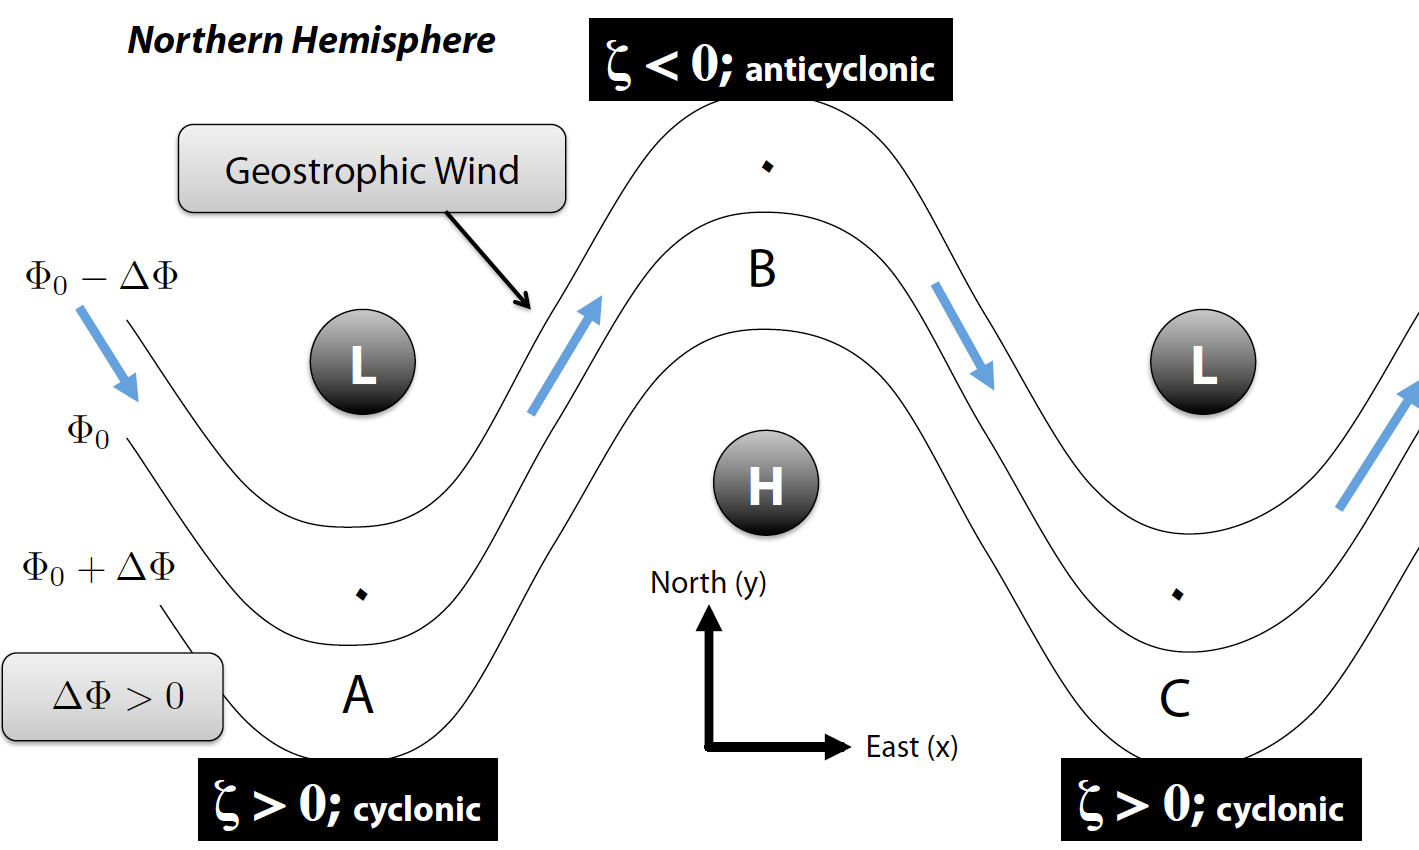
\includegraphics[width=0.65\textwidth]{images/ch05/p79_img01.png}
  \caption{Upper-tropospheric wave pattern on a $\beta$-plane showing
    geopotential contours (thin lines) with troughs (L, cyclonic,
    $\zeta > 0$) and ridges (H, anticyclonic, $\zeta < 0$).
    The geostrophic wind blows along the contours; arrows indicate the
    wind direction.  The $\beta$-effect and relative vorticity advection
    compete to determine the net wave propagation direction.
    \hisu{$\beta$-평면 위의 상층 파동 패턴.  기압골(L, $\zeta>0$)과
          기압능(H, $\zeta<0$)의 배치 및 지균풍 방향.}}
  \label{fig:upper-wave-LH}
\end{figure}

\begin{figure}[htbp]
  \centering
  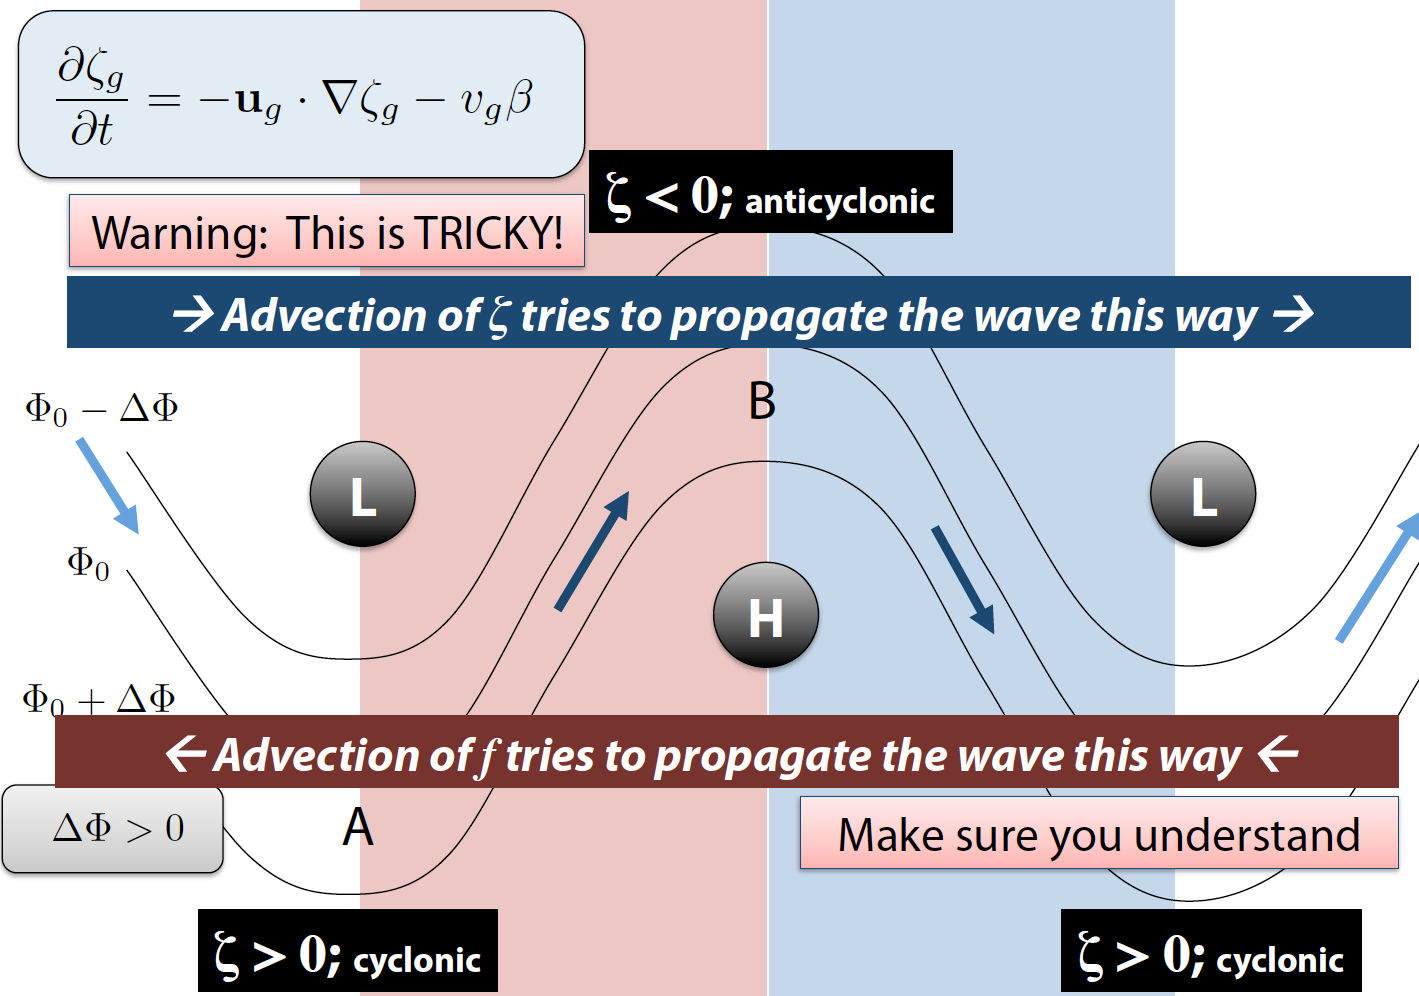
\includegraphics[width=0.65\textwidth]{images/ch05/p84_img01.png}
  \caption{Competition between relative vorticity advection (eastward
    propagation) and planetary vorticity advection (westward propagation).
    For \textgr{short waves}, relative vorticity advection dominates and the
    wave propagates eastward; for \textgr{long waves}, planetary vorticity
    advection dominates and the wave retrogresses westward.
    \hisu{상대 소용돌이도 이류(동진)와 행성 소용돌이도 이류(서진)의 경쟁.
          단파는 동진, 장파는 서진.  이 경쟁이 파동 전파 방향을 결정한다.}}
  \label{fig:vorticity-advection-competition}
\end{figure}

\begin{hisublock}
정상파 조건: $k^2 + l^2 = \beta/\bar{u}$

이 조건을 만족하는 파수의 파동만이 지형이나 가열에 의해 강제되어
시간 평균적으로 제자리에 머물 수 있다.
$\bar{u}$가 크면 정상파의 파수가 작아져서 (파장이 길어져서) 소수의 긴 파동만
정상일 수 있다.  이것이 중위도 대기의 planetary wave 패턴을 결정한다.
\end{hisublock}

% --------------------------------------------------------------------------
\subsection{QG Geopotential Tendency Equation (p-coordinate)}
\label{subsec:geopot-tendency}
% --------------------------------------------------------------------------

\textgr{Geopotential tendency}를 다음과 같이 정의한다:
\begin{equation}\label{eq:chi-def}
  \chi \equiv \frac{\partial\Phi}{\partial t}.
\end{equation}

\noindent
Pressure coordinates에서의 QG PV conservation으로부터 다음을 얻는다:

\begin{equation}\label{eq:geopot-tendency}
  \boxed{
  \underbrace{
    \left[\nabla^2
    + \frac{\partial}{\partial p}
      \!\left(\frac{f_0^2}{\sigma}\frac{\partial}{\partial p}\right)
    \right]\chi
  }_{\text{Term A (tendency)}}
  = \underbrace{
    -f_0\,\mathbf{V}_g\cdot\nabla
    \!\left(\frac{1}{f_0}\nabla^2\Phi + f\right)
  }_{\text{Term B (vorticity advection)}}
  \underbrace{
    -\frac{\partial}{\partial p}
    \!\left[-\frac{f_0^2}{\sigma}\,
      \mathbf{V}_g\cdot\nabla
      \!\left(-\frac{\partial\Phi}{\partial p}\right)
    \right]
  }_{\text{Term C (thickness advection)}}.
  }
\end{equation}

\begin{remark}[Interpretation of Terms]
\begin{itemize}
  \item \textgr{Term A}: An elliptic operator acting on the tendency $\chi$.
        Since $\nabla^2\chi \sim -\chi$ at the centre of an anomaly (as for
        any Laplacian), the sign of $\chi$ is \emph{opposite} to the sign of
        the right-hand side.
  \item \textgr{Term B --- Absolute vorticity advection}: Advection of
        absolute vorticity by the geostrophic wind.
        Positive (cyclonic) vorticity advection → $\chi < 0$ → geopotential
        \textgr{falls} → deepening low.
  \item \textgr{Term C --- Differential thickness advection}: Vertical
        derivative of the geostrophic temperature advection weighted by
        $f_0^2/\sigma$.  Warm advection increasing with height →
        $\chi < 0$ → geopotential falls.
\end{itemize}
\end{remark}

\begin{hisublock}
일기예보에서의 활용:
\begin{itemize}
  \item Term B: 500\,hPa 절대 소용돌이도 이류 지도에서 양의 AVA 지역 → 기압골 접근, 지상 기압 하강
  \item Term C: 1000--500\,hPa 두께 이류 → 온난 이류 증가 지역에서 지상 저기압 발달
  \item 두 항이 같은 위치에서 협력하면 → 급속한 저기압 발달 (explosive cyclogenesis)
\end{itemize}
\end{hisublock}

\begin{figure}[htbp]
  \centering
  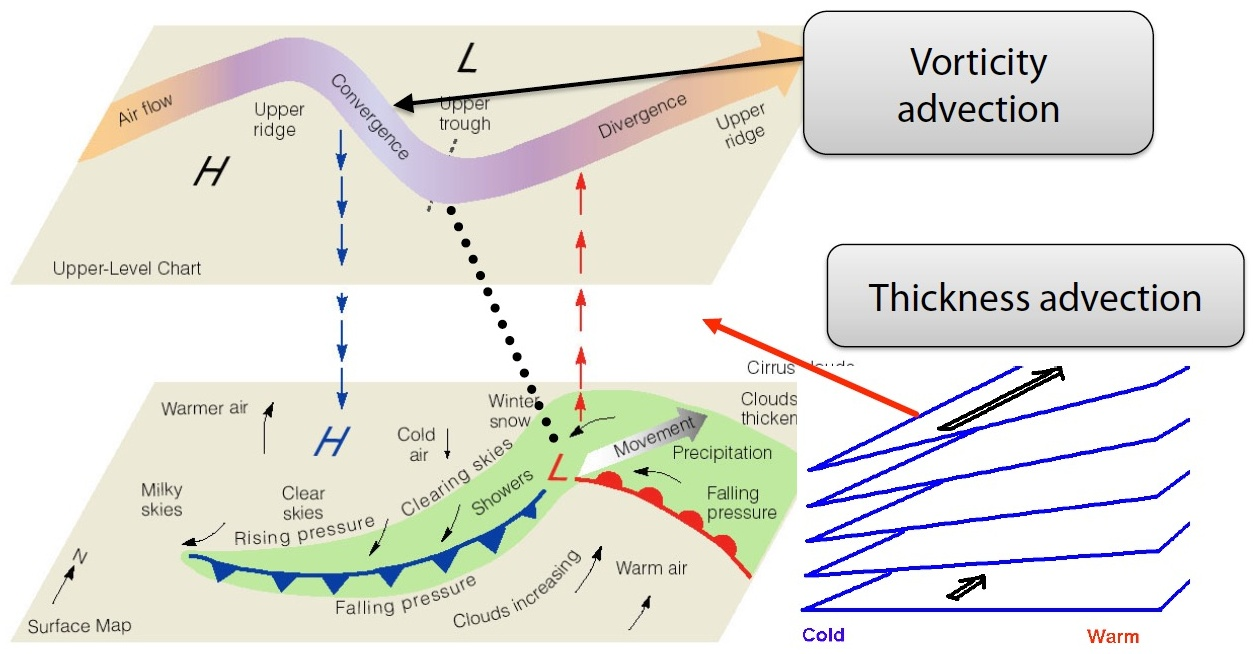
\includegraphics[width=0.65\textwidth]{images/ch05/p110_img01.jpeg}
  \caption{Relationship between the geopotential tendency equation forcing
    terms and synoptic weather patterns.  Upper panel: 500\,hPa chart
    showing vorticity advection (Term~B) downstream of the upper trough.
    Lower panel: surface map with thickness advection (Term~C) indicated
    by the thermal wind vectors.  Where positive vorticity advection and
    warm advection increasing with height coincide, rapid surface
    development occurs.
    \hisu{지위 고도 경향 방정식의 강제항과 일기도의 관계.
          상층 소용돌이도 이류(Term~B)와 두께 이류(Term~C)가 겹치는 곳에서
          지표 저기압이 급속히 발달한다.}}
  \label{fig:geopot-tendency-forcing}
\end{figure}

% --------------------------------------------------------------------------
\subsection{QG PV in Pressure Coordinates}\label{subsec:qgpv-p}
% --------------------------------------------------------------------------

Pressure coordinates에서의 vorticity와 stretching 기여를 모으면:

\begin{definition}[QG Potential Vorticity, $p$-coordinate]
\begin{equation}\label{eq:qgpv-p}
  \boxed{
  Q = \frac{1}{f_0}\nabla^2\Phi + f
    + \frac{\partial}{\partial p}
      \!\left(\frac{f_0}{\sigma}\frac{\partial\Phi}{\partial p}\right).
  }
\end{equation}
The three terms are:
\begin{enumerate}
  \item $\dfrac{1}{f_0}\nabla^2\Phi$: geostrophic relative vorticity
  \item $f = f_0 + \beta y$: planetary vorticity (Coriolis parameter)
  \item $\dfrac{\partial}{\partial p}\!\left(\dfrac{f_0}{\sigma}
        \dfrac{\partial\Phi}{\partial p}\right)$: stretching vorticity
\end{enumerate}
\end{definition}

\hisu{$p$-좌표 QG PV도 지위고도($\Phi$) 하나로 완전히 결정됨.  PV 역전(inversion)의 기초!}

% --------------------------------------------------------------------------
\subsection{QG Omega Equation (p-coordinate)}\label{subsec:omega-eq-p}
% --------------------------------------------------------------------------

Pressure coordinates에서의 omega equation은 vorticity equation \eqref{eq:qg-vort-p}과
thermodynamic equation \eqref{eq:qg-thermo-p} 사이에서 tendency $\chi$를
소거하여 얻는다.

\textit{Step 1.}  Apply $(\partial/\partial p)(f_0^2/\sigma)\cdot(\cdot)$
to the vorticity equation to get the stretching contribution to the tendency.

\textit{Step 2.}  Apply $\nabla^2$ to the thermodynamic equation.

\textit{Step 3.}  Subtract to eliminate $\partial\Phi/\partial t$ terms.

\noindent
그 결과가 \textgr{QG omega equation}이다:

\begin{equation}\label{eq:omega-p}
  \boxed{
  \underbrace{
    \left(\nabla^2 + \frac{f_0^2}{\sigma}\frac{\partial^2}{\partial p^2}\right)
    \omega
  }_{\text{Term A}}
  = \underbrace{
    \frac{f_0}{\sigma}\frac{\partial}{\partial p}
    \!\left[\mathbf{V}_g\cdot\nabla
      \!\left(\frac{1}{f_0}\nabla^2\Phi + f\right)
    \right]
  }_{\text{Term B}}
  + \underbrace{
    \frac{1}{\sigma}\nabla^2
    \!\left[\mathbf{V}_g\cdot\nabla
      \!\left(-\frac{\partial\Phi}{\partial p}\right)
    \right]
  }_{\text{Term C}}.
  }
\end{equation}

\begin{remark}[Interpretation of the Omega Equation]
\begin{itemize}
  \item \textgr{Term A}: Elliptic operator on $\omega$.
        Since $\nabla^2\omega \sim -\omega$ at the centre of a vertical velocity
        anomaly, the sign of $\omega$ is \textgr{opposite} to the sign of
        (B $+$ C).  Recall that in $p$-coordinates, $\omega < 0$ means
        \textgr{upward motion}.
  \item \textgr{Term B --- Differential vorticity advection}:
        Vertical derivative of absolute vorticity advection.
        \begin{itemize}
          \item Cyclonic vorticity advection increasing with height
                ($\partial/\partial p [\text{AVA}] < 0$ since $p$ decreases upward)
                → $\omega < 0$ → \textgr{ascent}.
          \item Physically: upper-level PV advection produces divergence aloft,
                requiring compensating ascent through the column.
        \end{itemize}
  \item \textgr{Term C --- Laplacian of thickness advection}:
        Laplacian of temperature advection by the geostrophic wind.
        \begin{itemize}
          \item Warm advection at a local maximum
                ($\nabla^2[\text{warm adv.}] < 0$)
                → $\omega < 0$ → \textgr{ascent} in the warm front region.
          \item Cold advection at a local maximum
                → $\omega > 0$ → \textgr{descent} behind the cold front.
        \end{itemize}
\end{itemize}
\end{remark}

\hisu{Term B: 상층에서 양의 소용돌이도 이류가 증가 → 상승.  Term C: 온난전선 → 상승, 한랭전선 뒤 → 하강.}

\begin{figure}[htbp]
  \centering
  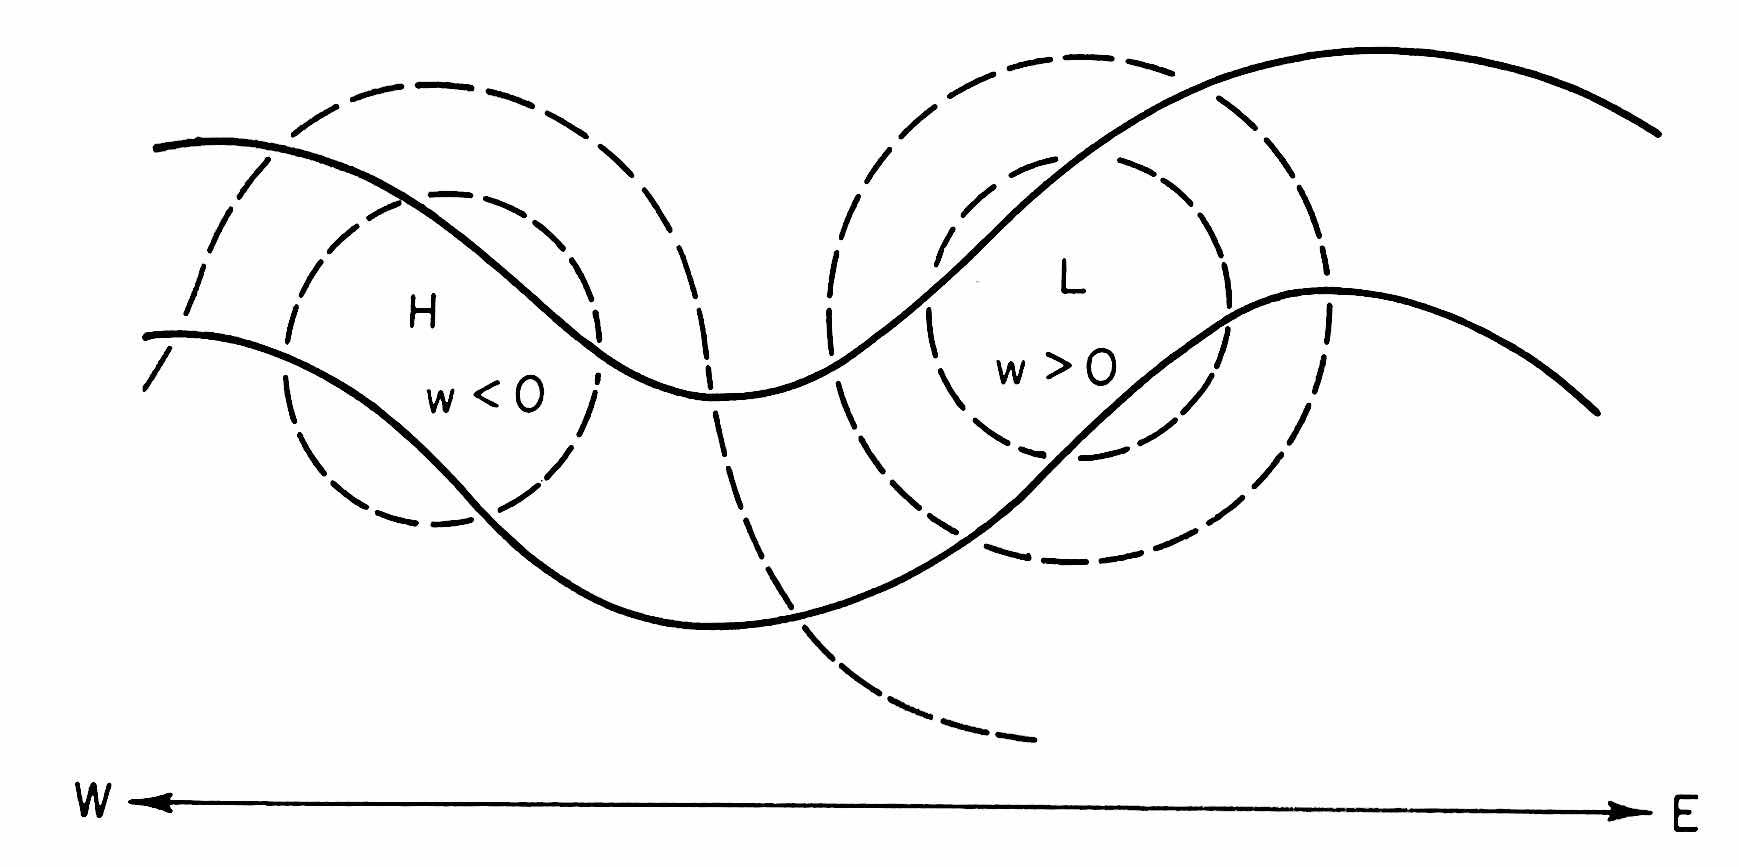
\includegraphics[width=0.65\textwidth]{images/ch05/p125_img01.jpeg}
  \caption{Schematic plan view of upper-level (solid) and lower-level
    (dashed) geopotential contours for a developing baroclinic wave.
    H marks the high (ridge) and L marks the low (trough).  Descending
    motion ($w < 0$) occurs in the high-pressure region; ascending motion
    ($w > 0$) occurs in the low-pressure region.  The westward tilt with
    height between the upper and lower wave patterns is evident.
    \hisu{발달 중인 경압파의 상층(실선)--하층(점선) 지위고도 등치선.
          고기압 영역에서 하강($w<0$), 저기압 영역에서 상승($w>0$).}}
  \label{fig:upper-lower-wave-vertical-motion}
\end{figure}

\begin{figure}[htbp]
  \centering
  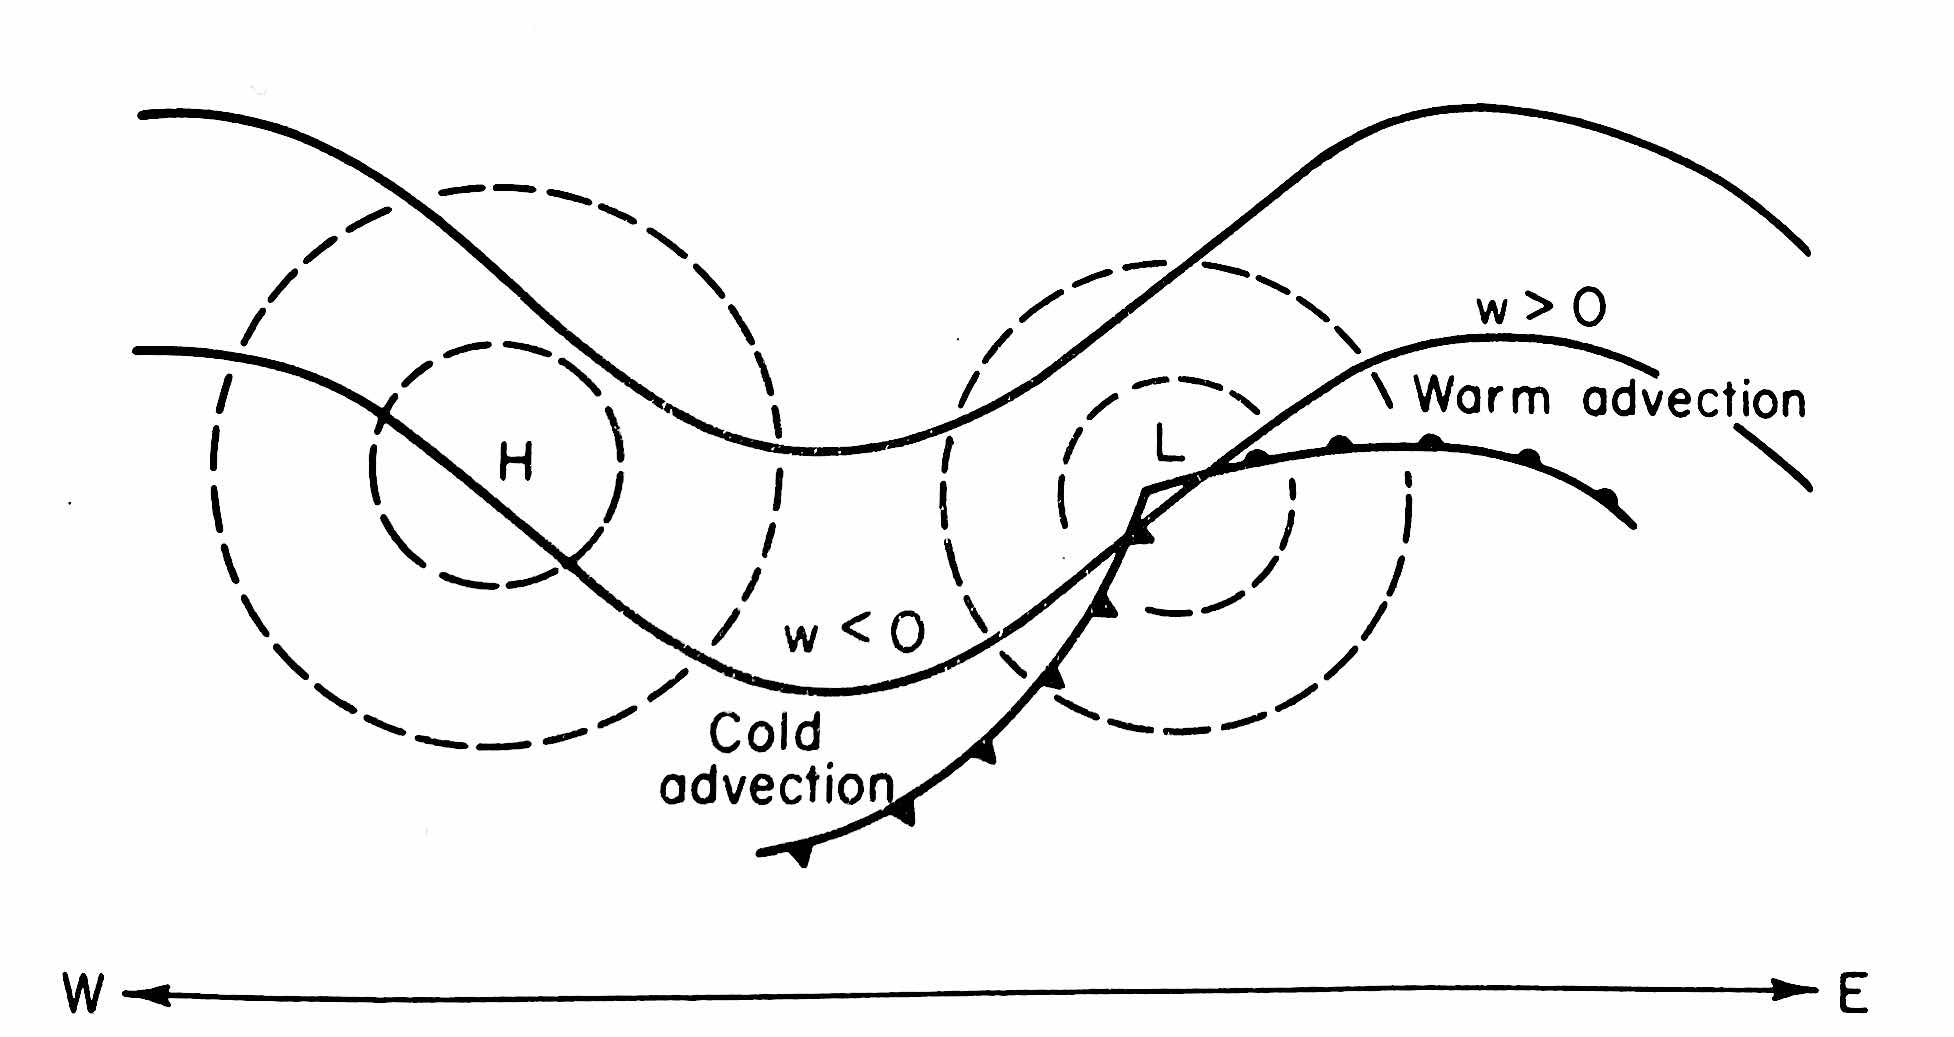
\includegraphics[width=0.65\textwidth]{images/ch05/p129_img01.jpeg}
  \caption{As in Fig.~\ref{fig:upper-lower-wave-vertical-motion} but with
    frontal boundaries and temperature advection indicated.  Warm advection
    ($w > 0$, ascent) occurs ahead of the surface low where the warm front
    lifts warm air over cold air; cold advection ($w < 0$, descent) occurs
    behind the low.  This pattern is consistent with the omega-equation
    forcing by the Laplacian of temperature advection (Term~C).
    \hisu{전선과 온도 이류가 표시된 경압파 평면도.
          온난 전선 → 상승(온난 이류), 한랭 전선 뒤 → 하강(한랭 이류).
          오메가 방정식 Term~C의 강제에 해당.}}
  \label{fig:wave-temp-advection}
\end{figure}

\begin{hisublock}
오메가 방정식의 실용적 중요성:
\begin{itemize}
  \item $\omega$는 직접 측정이 거의 불가능 → 반드시 진단 방정식으로 계산
  \item Term B는 주로 상층 일기도(500/300\,hPa)의 트로프/릿지 패턴에서 추정
  \item Term C는 지표 전선 구조와 두께 이류 패턴에서 추정
  \item 상승 운동 → 구름, 강수 → 일기예보의 핵심!
\end{itemize}
\end{hisublock}

% --------------------------------------------------------------------------
\subsection{Barotropic vs.\ Baroclinic Atmosphere}\label{subsec:baro}
% --------------------------------------------------------------------------

Barotropic 대기와 baroclinic 대기의 구분은
QG dynamics와 불안정의 본질을 이해하는 데 핵심적이다.

\begin{definition}[Barotropic Atmosphere]
A fluid is \textbf{barotropic} if density depends only on pressure:
$\rho = \rho(p)$.  Equivalently, isobaric surfaces and isopycnal (constant
density) surfaces are \textgr{parallel}.  Consequences:
\begin{itemize}
  \item No horizontal temperature gradients on pressure surfaces.
  \item No thermal wind: $\partial\mathbf{V}_g/\partial z = 0$, so the
        geostrophic wind is independent of height.
  \item No available potential energy (APE) to convert: the atmosphere is
        in its minimum-PE state.
\end{itemize}
\hisu{순압 대기: 등압면과 등밀도면이 평행 → 바람이 고도에 따라 변하지 않음}
\end{definition}

\begin{definition}[Baroclinic Atmosphere]
A fluid is \textbf{baroclinic} if density depends on both pressure and
temperature: $\rho = \rho(p, T)$.  Equivalently, isobaric surfaces and
isothermal/isopycnal surfaces \textgr{tilt relative to each other}.
Consequences:
\begin{itemize}
  \item Horizontal temperature gradients exist on pressure surfaces.
  \item The thermal wind relation gives nonzero vertical wind shear:
        $\partial\mathbf{V}_g/\partial z \neq 0$.
  \item Available potential energy (APE) exists and can be converted to
        kinetic energy through baroclinic instability.
\end{itemize}
\hisu{경압 대기: 등압면과 등온면이 기울어져 있음 → 위치에너지를 운동에너지로 변환 가능!}
\end{definition}

\begin{figure}[htbp]
  \centering
  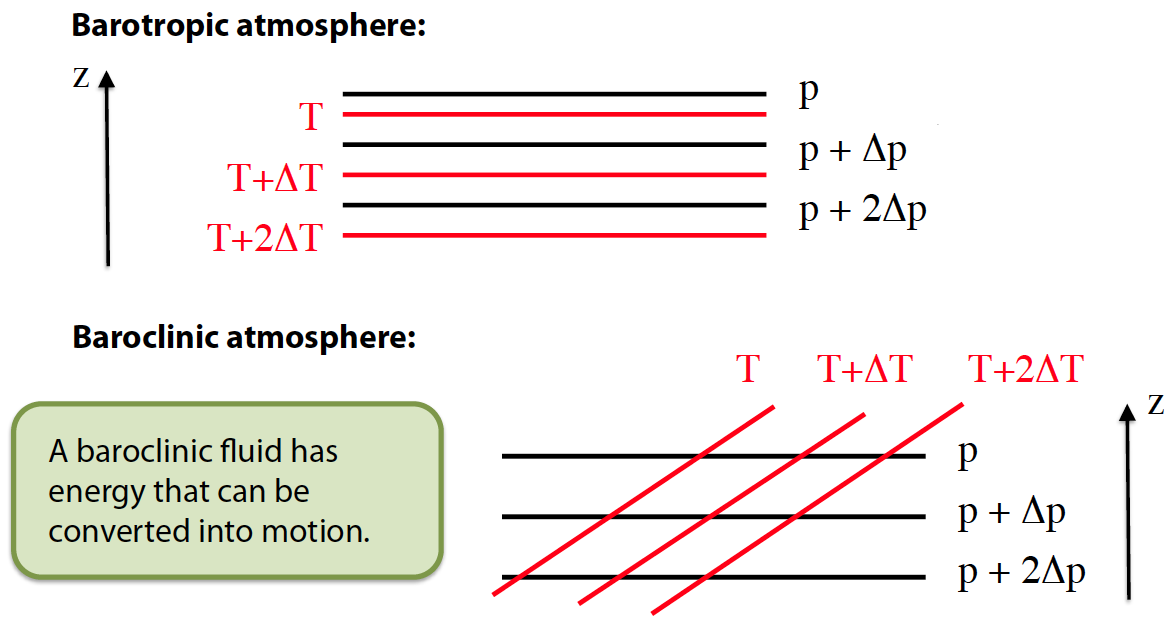
\includegraphics[width=0.65\textwidth]{images/ch05/p116_img01.png}
  \caption{Comparison of barotropic and baroclinic atmospheres.
    Top: in a \textgr{barotropic} atmosphere, isobaric surfaces (black)
    and isothermal surfaces (red) are parallel --- no horizontal
    temperature gradient on pressure surfaces, no vertical wind shear,
    and no available potential energy (APE).
    Bottom: in a \textgr{baroclinic} atmosphere, isobaric and isothermal
    surfaces are tilted relative to each other --- horizontal temperature
    gradients exist, the thermal wind produces vertical shear, and APE
    is available for conversion to kinetic energy via baroclinic instability.
    \hisu{순압 대기 vs.\ 경압 대기.  순압: 등압면과 등온면이 평행 (APE\,=\,0).
          경압: 등압면과 등온면이 기울어져 있어 에너지 변환이 가능.}}
  \label{fig:barotropic-baroclinic}
\end{figure}

\begin{hisublock}
순압 vs.\ 경압의 핵심 차이:
\begin{multicols}{2}
\textbf{순압 (Barotropic)}
\begin{itemize}
  \item $\rho = \rho(p)$ only
  \item $\partial\mathbf{V}_g/\partial z = 0$
  \item APE = 0
  \item 경압 불안정 없음
  \item 순압 불안정만 가능
\end{itemize}
\columnbreak
\textbf{경압 (Baroclinic)}
\begin{itemize}
  \item $\rho = \rho(p, T)$
  \item $\partial\mathbf{V}_g/\partial z \neq 0$
  \item APE $> 0$
  \item 경압 불안정 가능
  \item 중위도 종관 시스템의 원동력
\end{itemize}
\end{multicols}
실제 대기는 항상 경압적이다 --- 적도-극 온도 경도가 존재하기 때문.
순압 대기는 이론적 이상화에 불과하지만, 성층권이나 열대 대기의 일부 측면을
이해하는 데 유용하다.
\end{hisublock}

\begin{hisublock}
\textbf{참고 문헌 가이드:}
\begin{itemize}
  \item Holton \& Hakim Ch.~6 -- $p$-좌표 QG equations 전체 체계
  \item Marshall \& Plumb (2008), \textit{Atmosphere, Ocean, and Climate Dynamics}, Ch.~8.2.2 (pp.~145--148, PDF pp.~166--169) -- extratropical circulation의 QG 해석
  \item Peixoto \& Oort (1992), \textit{Physics of Climate}, Ch.~14.5 (book pp.~385--392; 본 PDF에는 목차만 수록) -- EP flux와 파동-평균류 상호작용
  \item Vallis Ch.~5.4--5.6 -- Rossby waves와 QG 파동 역학
\end{itemize}
\end{hisublock}


% =============================================================================
\section{Summary of QG Equations}\label{sec:qg-summary}
% =============================================================================

참고의 편의를 위해 두 좌표계에서의 QG equations 전체를 모아 정리한다.

% --------------------------------------------------------------------------
\subsection{QG System in $z$-coordinates (Boussinesq)}
% --------------------------------------------------------------------------

\begin{enumerate}
  \item \textbf{Geostrophic wind}:
    $\displaystyle \mathbf{V}_g = \frac{1}{\rho_0 f}\,\hat{k}\times\nabla p$

  \item \textbf{Thermal wind}:
    $\displaystyle \frac{\partial\mathbf{V}_g}{\partial z}
    = \frac{g}{f\theta_0}\,\hat{k}\times\nabla\theta$

  \item \textbf{QG vorticity equation}:
    $\displaystyle \frac{d}{dt}(\zeta_g + f) = f\frac{\partial w}{\partial z}$

  \item \textbf{QG thermodynamic equation}:
    $\displaystyle \frac{d\theta}{dt} = -w\frac{d\theta_0}{dz}$

  \item \textbf{QG PV conservation}:
    $\displaystyle \frac{dQ}{dt} = 0$,
    \quad $Q = (\zeta_g + f) + f\dfrac{\partial}{\partial z}
    \!\left(\dfrac{\theta}{d\theta_0/dz}\right)$

  \item \textbf{Omega equation}:
    $\displaystyle \left(\nabla^2 + \frac{f^2}{N^2}
    \frac{\partial^2}{\partial z^2}\right) w
    = \frac{g}{\theta_0 N^2}\nabla^2(-\mathbf{V}_g\cdot\nabla\theta)
    - \frac{f}{N^2}\frac{\partial}{\partial z}
    (-\mathbf{V}_g\cdot\nabla\zeta_g)$
\end{enumerate}

% --------------------------------------------------------------------------
\subsection{QG System in $p$-coordinates}
% --------------------------------------------------------------------------

\begin{enumerate}
  \item \textbf{Geostrophic wind}:
    $\displaystyle u_g = -\frac{1}{f_0}\frac{\partial\Phi}{\partial y}$,
    \quad $v_g = \frac{1}{f_0}\frac{\partial\Phi}{\partial x}$

  \item \textbf{QG momentum equation}:
    $\displaystyle \frac{d\mathbf{V}_g}{dt}
    = -f_0\hat{k}\times\mathbf{V}_a - \beta y\hat{k}\times\mathbf{V}_g$

  \item \textbf{QG vorticity equation}:
    $\displaystyle \frac{d\zeta_g}{dt}
    = -\mathbf{V}_g\cdot\nabla(\zeta_g + f)
    + f_0\frac{\partial\omega}{\partial p}$

  \item \textbf{QG thermodynamic equation}:
    $\displaystyle \left(\frac{\partial}{\partial t}
    + \mathbf{V}_g\cdot\nabla\right)
    \!\left(-\frac{\partial\Phi}{\partial p}\right)
    - \sigma\omega = \frac{\kappa J}{p}$

  \item \textbf{QG PV conservation}:
    $\displaystyle \frac{dQ}{dt} = 0$,
    \quad $Q = \frac{1}{f_0}\nabla^2\Phi + f
    + \frac{\partial}{\partial p}
    \!\left(\frac{f_0}{\sigma}\frac{\partial\Phi}{\partial p}\right)$

  \item \textbf{Geopotential tendency equation}:
    See Eq.~\eqref{eq:geopot-tendency}

  \item \textbf{Omega equation}:
    See Eq.~\eqref{eq:omega-p}
\end{enumerate}

\hisu{이 요약표를 시험 전에 반드시 외울 것!  QG 체계의 모든 것이 여기에 있다.}

\begin{hisublock}
QG 이론의 핵심 메시지 요약:
\begin{enumerate}
  \item QG PV 하나가 전체 역학을 지배한다 ($dQ/dt = 0$).
  \item 모든 동역학 변수는 단일 스칼라 장 ($p$ 또는 $\Phi$)으로 결정된다 (PV 역전).
  \item 연직 운동과 지위 고도 변화는 소용돌이도 이류와 온도 이류로 진단된다.
  \item 단파는 동진, 장파는 서진 --- 정상파는 $K_s = \sqrt{\beta/\bar{u}}$.
  \item 경압 불안정은 APE를 KE로 전환하며, 서쪽 기울기가 필수적이다.
\end{enumerate}
Ref: Holton and Hakim, Ch.~6; Vallis, \textit{Atmospheric and Oceanic Fluid Dynamics}, Ch.~5.
\end{hisublock}
